\documentclass[aspectratio=169,10pt]{beamer}

\usepackage[utf8]{inputenc}
\usepackage{amsmath,amssymb,amsfonts,bm,mathtools}
\usepackage{graphicx}
\usepackage{booktabs}
\usepackage{tikz}
\usepackage{xcolor}

% -----------------------------------------------------------------------------
% Professional Clean Styling (Madrid base with custom Teal & Navy palette)
% -----------------------------------------------------------------------------
\usetheme{Madrid}
\usefonttheme{professionalfonts}

\definecolor{DeepNavy}{RGB}{20, 35, 60}
\definecolor{TealAccent}{RGB}{12, 120, 125}
\definecolor{SoftTeal}{RGB}{235, 245, 245}
\definecolor{AlertRed}{RGB}{205, 45, 45}
\definecolor{SafeGreen}{RGB}{35, 140, 60}
\definecolor{LightGray}{RGB}{245, 247, 250}

\setbeamercolor{palette primary}{bg=DeepNavy,fg=white}
\setbeamercolor{palette secondary}{bg=TealAccent,fg=white}
\setbeamercolor{palette tertiary}{bg=DeepNavy!80,fg=white}
\setbeamercolor{palette quaternary}{bg=DeepNavy,fg=white}
\setbeamercolor{structure}{fg=TealAccent}
\setbeamercolor{frametitle}{bg=DeepNavy,fg=white}
\setbeamercolor{title}{bg=DeepNavy,fg=white}

\setbeamercolor{block title}{bg=TealAccent,fg=white}
\setbeamercolor{block body}{bg=SoftTeal,fg=black}
\setbeamercolor{block title alerted}{bg=AlertRed,fg=white}
\setbeamercolor{block body alerted}{bg=AlertRed!10,fg=black}
\setbeamercolor{block title example}{bg=SafeGreen,fg=white}
\setbeamercolor{block body example}{bg=SafeGreen!10,fg=black}

\setbeamertemplate{navigation symbols}{}
\setbeamertemplate{footline}{
  \leavevmode%
  \hbox{%
  \begin{beamercolorbox}[wd=.333333\paperwidth,ht=2.25ex,dp=1ex,center]{author in head/foot}%
    \usebeamerfont{author in head/foot}\insertshortauthor
  \end{beamercolorbox}%
  \begin{beamercolorbox}[wd=.333333\paperwidth,ht=2.25ex,dp=1ex,center]{title in head/foot}%
    \usebeamerfont{title in head/foot}\insertshorttitle
  \end{beamercolorbox}%
  \begin{beamercolorbox}[wd=.333333\paperwidth,ht=2.25ex,dp=1ex,right]{date in head/foot}%
    \insertframenumber{} / \inserttotalframenumber\hspace*{2ex}
  \end{beamercolorbox}}%
  \vskip0pt%
}

% -----------------------------------------------------------------------------
% Title Information
% -----------------------------------------------------------------------------
\title[Control Barrier Functions (CBFs)]{\textbf{\LARGE Control Barrier Functions (CBFs)}}
\subtitle{A Beginner's Guide to Safety Filters in Autonomous Drone Navigation}
\title[Goal-Directed Velocity Control: APF vs. CBF]{\textbf{\LARGE Goal-Directed Navigation with Velocity Control}}
\subtitle{From Artificial Potential Fields (APF) to Control Barrier Functions (CBF)}
\author[Autonomous Aerial Systems]{Autonomous Aerial Systems Course}
\institute[Robotics \& Control]{Department of Robotics \& Intelligent Systems}
\date[\today]{Introductory Lecture}

\begin{document}

% =============================================================================
% Slide 1: Title Slide
% =============================================================================
\begin{frame}
  \titlepage
\end{frame}

% =============================================================================
% Slide 2: The Core Problem in Autonomous Robotics
% Slide 2: Velocity-Controlled Drone Navigation
% =============================================================================
\begin{frame}{The Dilemma: Performance vs. Safety}
\begin{frame}{Problem Formulation: High-Level Velocity as Control Input}
  \centering
  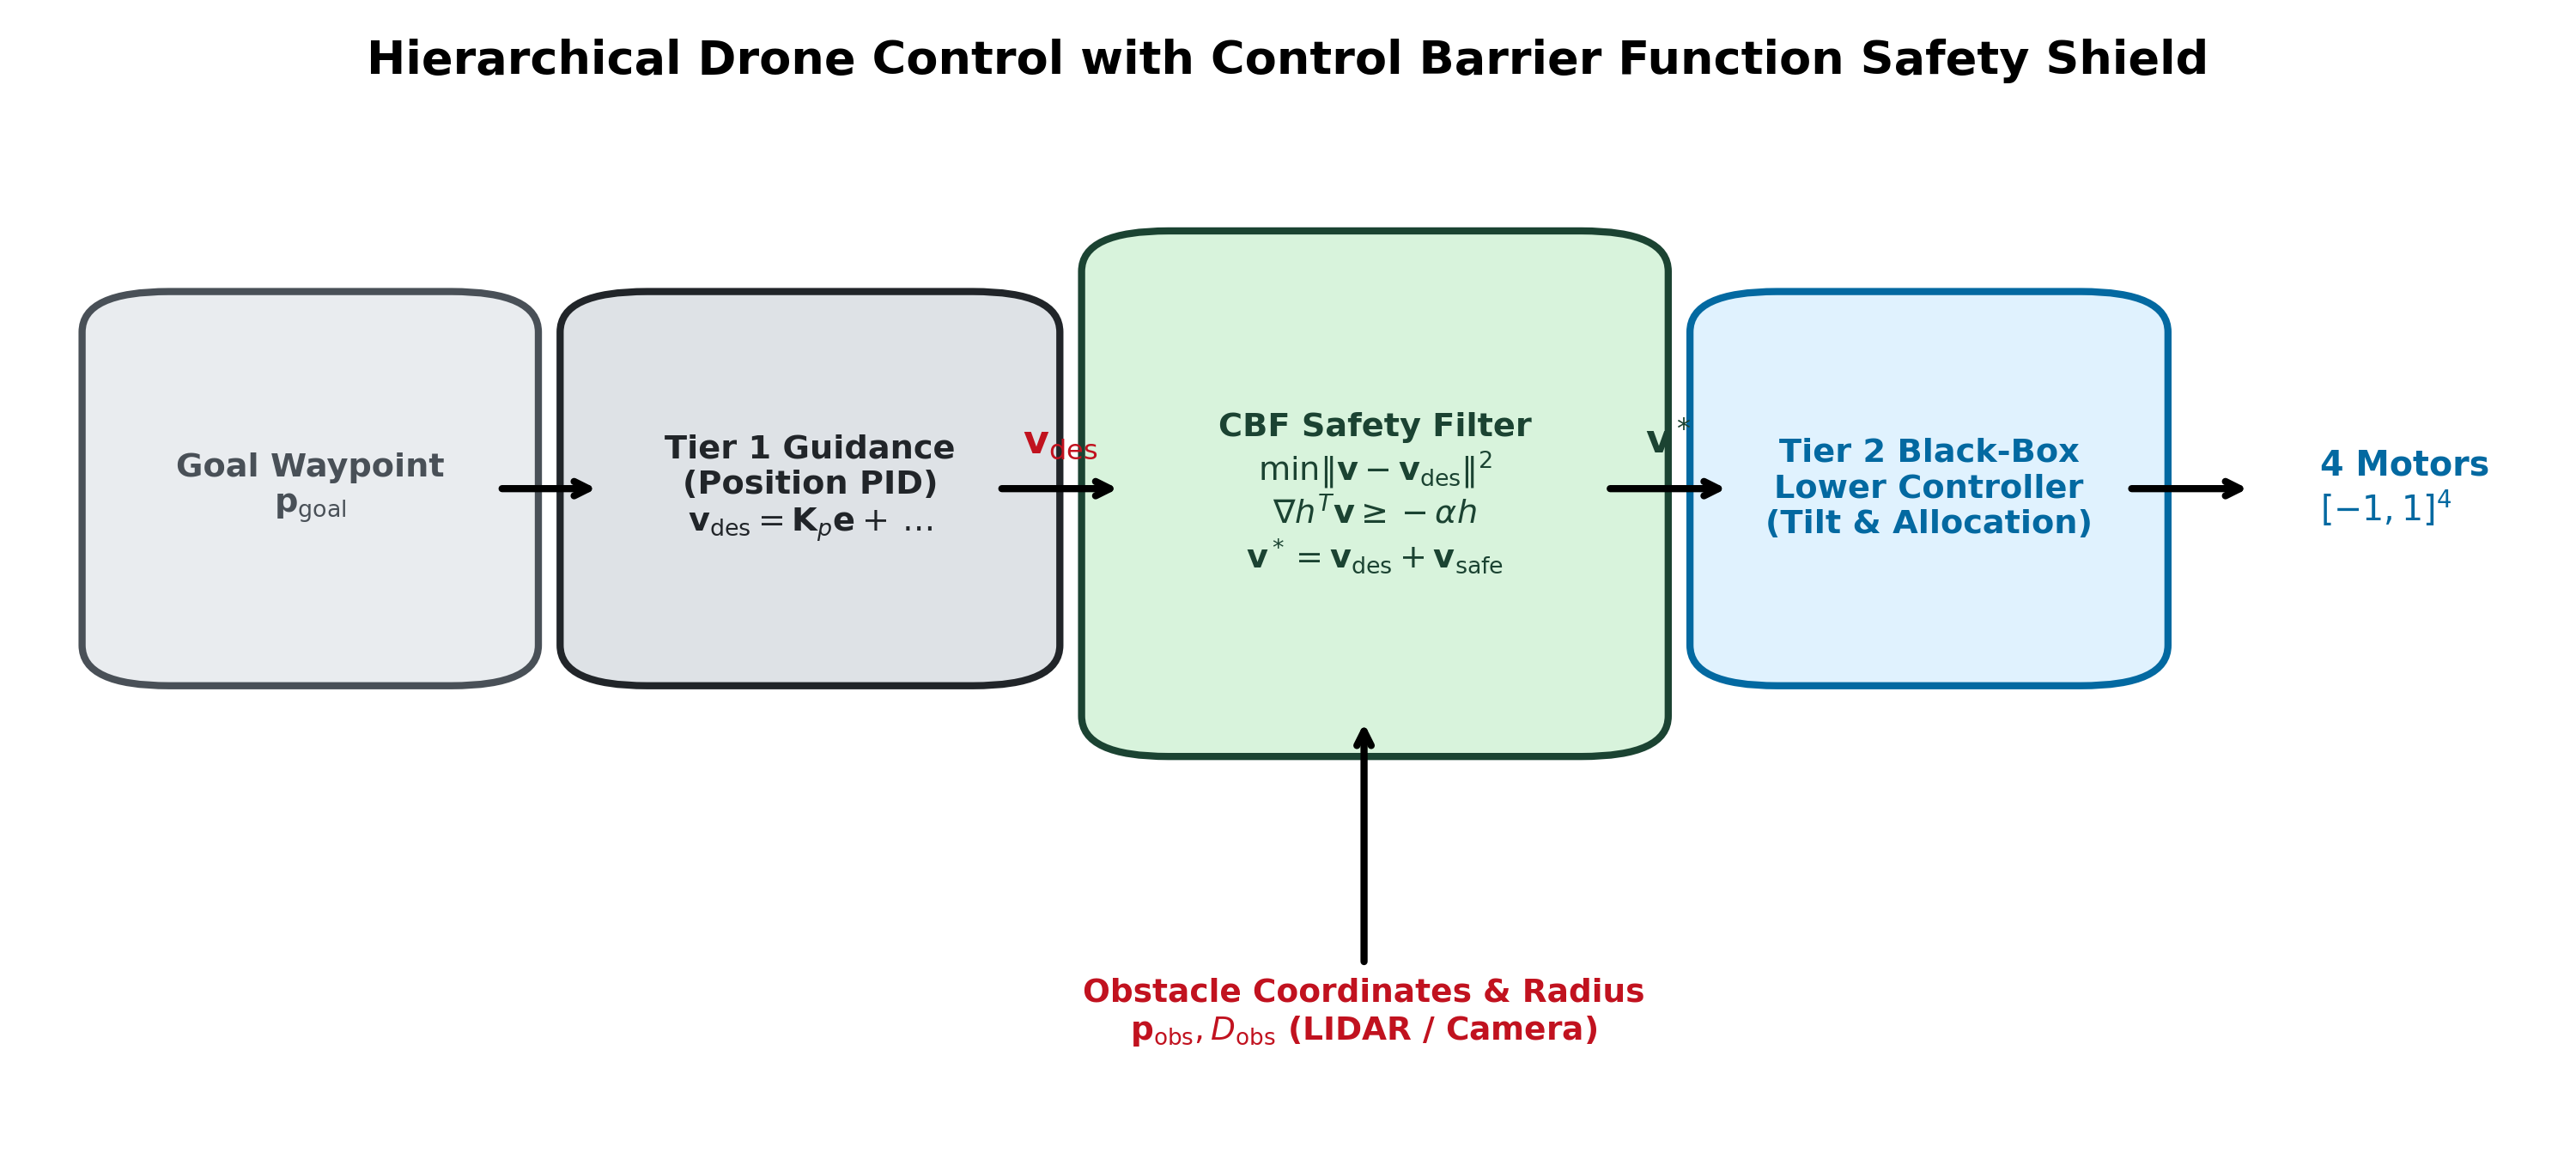
\includegraphics[height=0.32\textheight, keepaspectratio]{cbf_architecture_block.png}

  \vspace{0.2em}
  \begin{columns}[T]
    \begin{column}{0.54\textwidth}
      \textbf{Every autonomous robot juggles two competing goals:}
      \begin{enumerate}
        \item \textbf{Performance (Goal-Seeking)}:
    \begin{column}{0.48\textwidth}
      \begin{block}{Tier 1: Kinematic Guidance ($\dot{\mathbf{p}} = \mathbf{v}_{\mathrm{cmd}}$)}
        \small
        \begin{itemize}
          \item Follow a path, navigate to a waypoint, dock cleanly.
          \item Handled by a \textbf{Position PID} controller:
          $$\mathbf{v}_{\mathrm{des}} = \mathbf{K}_p (\mathbf{p}_{\mathrm{goal}} - \mathbf{p})$$
          \item Treats drone as a single integrator in $\mathbb{R}^3$.
          \item High-level controller outputs \textbf{velocity command} $\mathbf{v}_{\mathrm{cmd}}$.
          \item Objective: Navigate from $\mathbf{p}_0$ to $\mathbf{p}_{\mathrm{goal}}$ while avoiding obstacles at $\mathbf{p}_{\mathrm{obs}}$.
        \end{itemize}
        \item \textbf{Safety (Collision Avoidance)}:
      \end{block}
    \end{column}

    \begin{column}{0.48\textwidth}
      \begin{block}{Tier 2: 6-DOF Dynamic Tracking}
        \small
        \begin{itemize}
          \item Never collide with people, walls, or obstacles!
          \item Fast inner attitude loop (PID / SE(3)).
          \item Tilts drone (pitch $\theta$, roll $\phi$) to track $\mathbf{v}_{\mathrm{cmd}}$.
          \item Allocates motor thrusts $\Omega_{1,2,3,4} \in [-1, 1]^4$.
        \end{itemize}
      \end{enumerate}
      \end{block}
    \end{column}
  \end{columns}

      \vspace{0.1em}
      \begin{alertblock}{The ``Blind Driver'' Problem}
        \small Standard PID is \textbf{obstacle-blind}. If an obstacle sits between the drone and the goal, the PID commands full speed straight into the obstacle!
      \end{alertblock}
  \vspace{0.2em}
  \centering
  \footnotesize \textbf{The Core Question}: How do we compute $\mathbf{v}_{\mathrm{cmd}}$? We explore \textbf{two major paradigms}: APF vs. CBF.
\end{frame}

% =============================================================================
% Slide 3: Paradigm 1 - Artificial Potential Fields (APF)
% =============================================================================
\begin{frame}{Paradigm 1: Artificial Potential Fields (APF)}
  \begin{columns}[T]
    \begin{column}{0.54\textwidth}
      Classic approach (Khatib 1986): Robot rolls downhill on an energy landscape $U(\mathbf{p}) = U_{\mathrm{att}}(\mathbf{p}) + U_{\mathrm{rep}}(\mathbf{p})$:
      $$\mathbf{v}_{\mathrm{cmd}}^{\mathrm{APF}} = -\nabla U(\mathbf{p}) = \mathbf{v}_{\mathrm{att}}(\mathbf{p}) + \mathbf{v}_{\mathrm{rep}}(\mathbf{p})$$

      \begin{block}{Velocity Field Components}
        \small
        \textbf{Goal Attraction} (pulls toward target):
        $$\mathbf{v}_{\mathrm{att}}(\mathbf{p}) = -k_{\mathrm{att}} (\mathbf{p} - \mathbf{p}_{\mathrm{goal}})$$
        \textbf{Obstacle Repulsion} (pushes outward within $D_{\mathrm{obs}}$):
        $$\mathbf{v}_{\mathrm{rep}}(\mathbf{p}) = k_{\mathrm{rep}} \left(\frac{1}{d} - \frac{1}{D_{\mathrm{obs}}}\right) \frac{1}{d^2} \hat{\mathbf{n}}$$
        where $d = \|\mathbf{p} - \mathbf{p}_{\mathrm{obs}}\|$ and $\hat{\mathbf{n}} = \frac{\mathbf{p} - \mathbf{p}_{\mathrm{obs}}}{d}$.
      \end{block}
    \end{column}

    \begin{column}{0.44\textwidth}
      \centering
      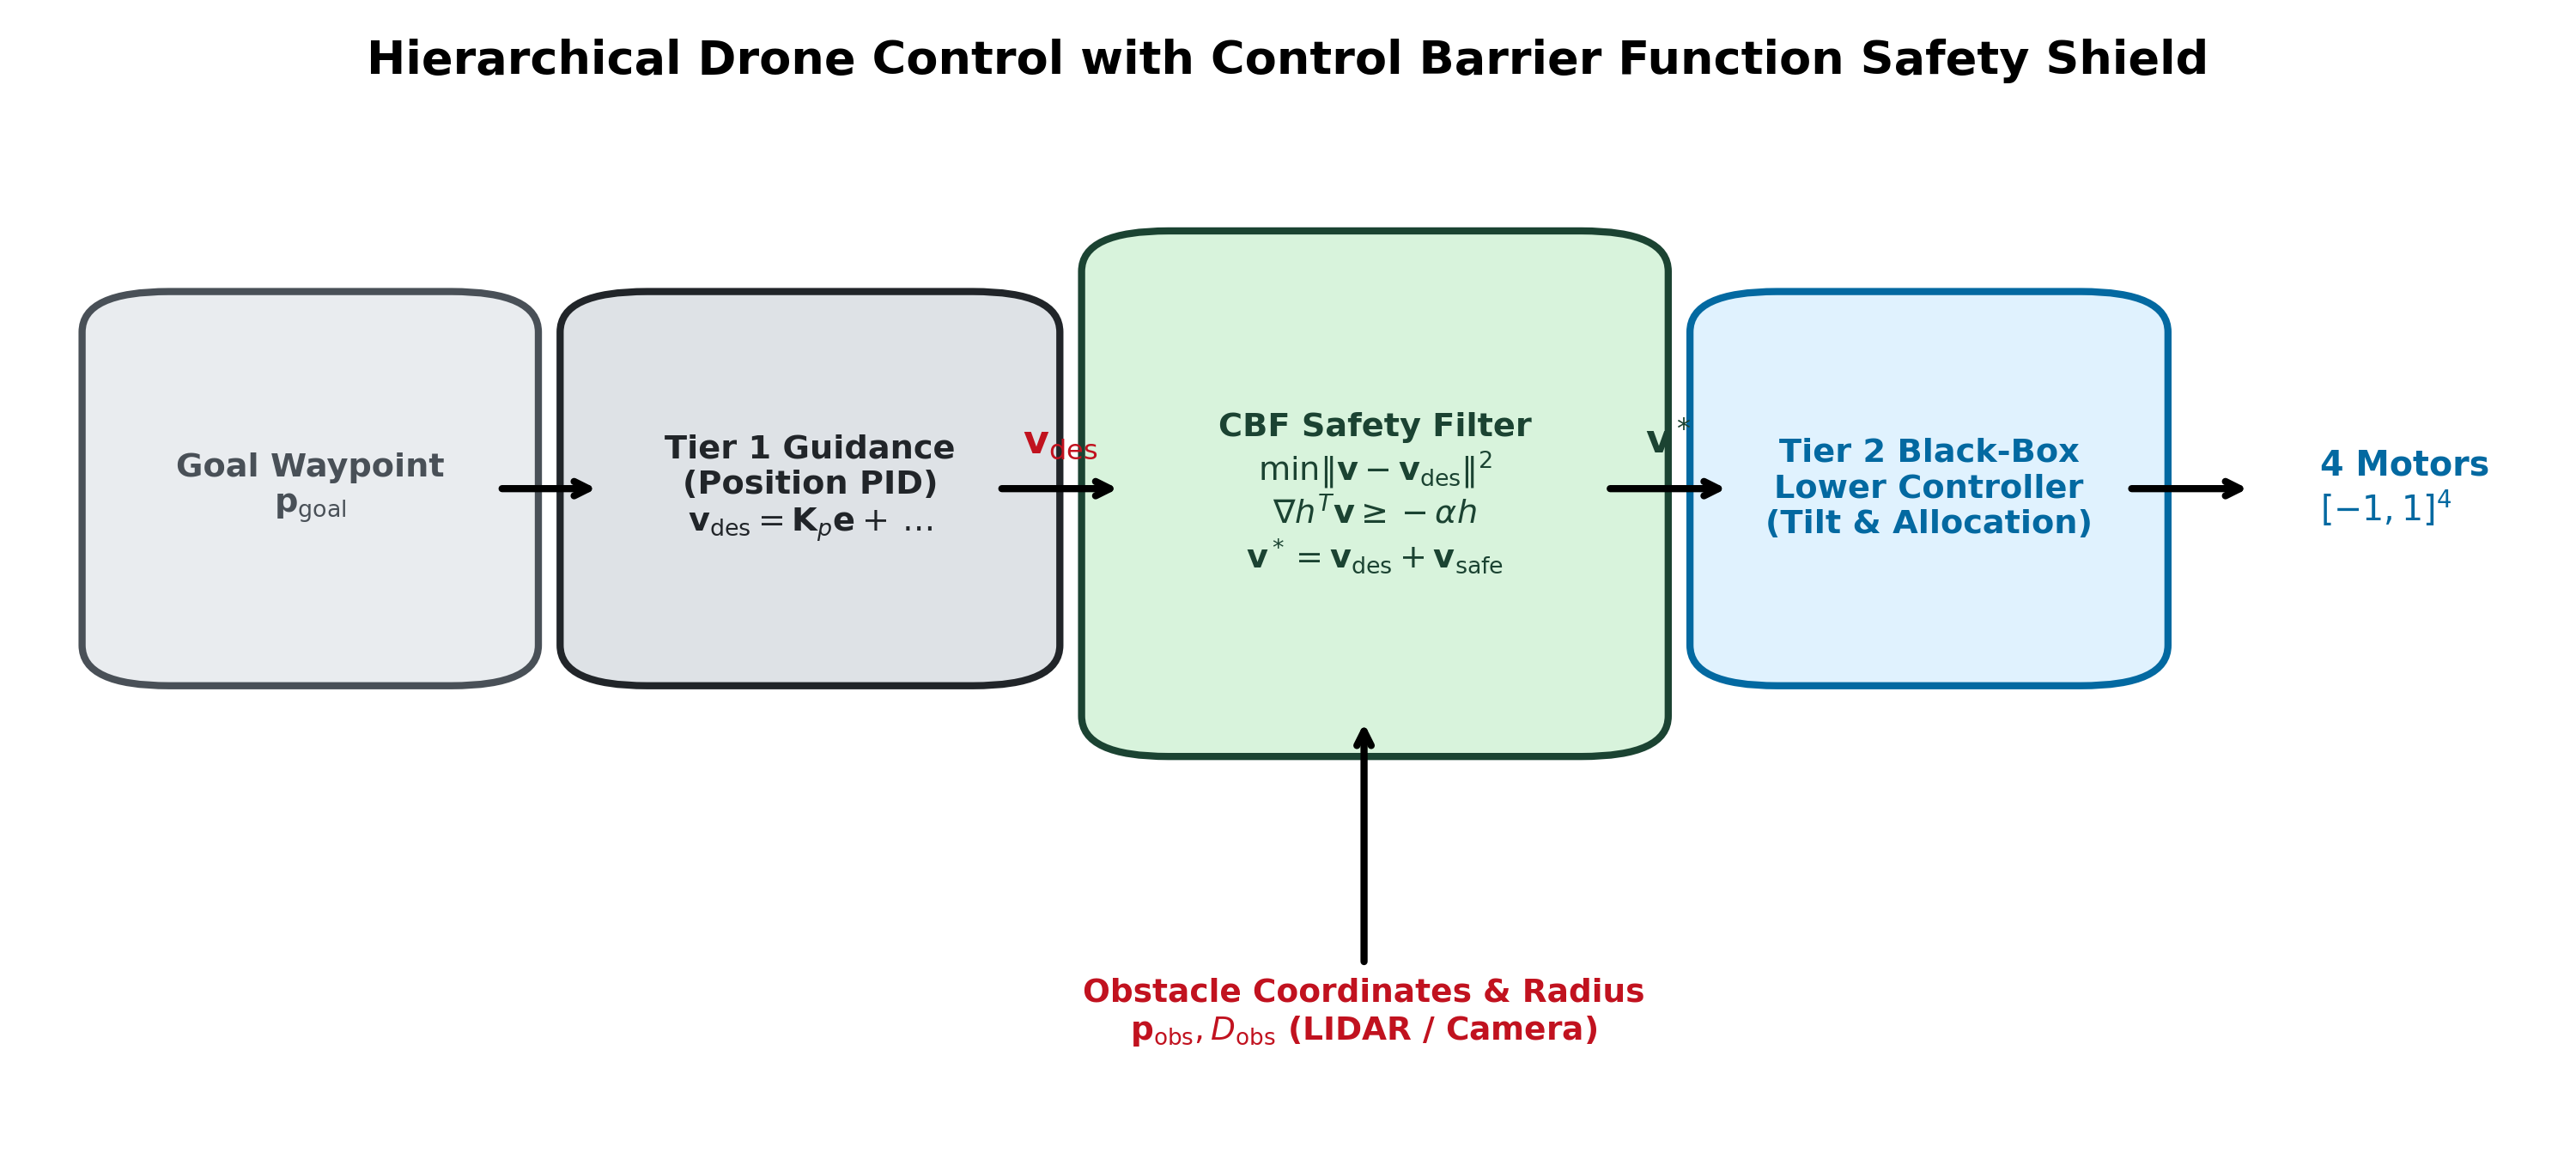
\includegraphics[width=\textwidth]{cbf_architecture_block.png}
      \begin{exampleblock}{The Appeal of APF}
        \small
        \begin{itemize}
          \item Very simple, closed-form vector sum.
          \item Intuitive physical analogy (charged particle attracted to goal and repelled by charges).
          \item Taught in robotics textbooks for 35+ years!
        \end{itemize}
      \end{exampleblock}

      \vspace{0.3em}
      \footnotesize \textbf{Our Mission Today}: Insert an intelligent \textbf{Safety Shield} between high-level guidance and drone motors.
      \begin{alertblock}{The Hidden Trap}
        \small APF \textbf{blends} goal tracking and safety into an unconstrained vector sum. This causes \textbf{four fatal failure modes} in practice!
      \end{alertblock}
    \end{column}
  \end{columns}
\end{frame}

% =============================================================================
% Slide 3: Why Artificial Potential Fields (APF) Fail
% Slide 4: APF Failures 1 & 2 - Deadlocks & GNRON
% =============================================================================
\begin{frame}{Historical Approach: Why Potential Fields Fail}
\begin{frame}{APF Failure Modes 1 \& 2: Stalling and Goal Inaccessibility}
  \begin{columns}[T]
    \begin{column}{0.52\textwidth}
      For decades, textbooks taught \textbf{Artificial Potential Fields (APF)}:
      $$\mathbf{F}_{\mathrm{net}} = \mathbf{F}_{\mathrm{attract}}(\mathbf{p}_{\mathrm{goal}}) + \mathbf{F}_{\mathrm{repulse}}(\mathbf{p}_{\mathrm{obs}})$$
    \begin{column}{0.50\textwidth}
      \begin{alertblock}{Failure 1: Collinear Deadlock (Local Minimum)}
        \scriptsize
        \begin{itemize}
          \item When start, obstacle, and goal align on a line:
          \item $\mathbf{v}_{\mathrm{att}}$ pulls forward; $\mathbf{v}_{\mathrm{rep}}$ pushes directly backward.
          \item At distance $d^*$, $\|\mathbf{v}_{\mathrm{att}}\| = \|\mathbf{v}_{\mathrm{rep}}\| \implies \mathbf{v}_{\mathrm{cmd}} = \mathbf{0}$.
          \item \textbf{The drone permanently freezes in mid-air!}
        \end{itemize}
      \end{alertblock}

      \vspace{0.1em}
      \begin{alertblock}{Fatal Flaws of Potential Fields in Practice}
        \small
      \begin{alertblock}{Failure 2: Goal Non-Reachable (GNRON)}
        \scriptsize
        \begin{itemize}
          \item \textbf{Local Minima Traps}: Attractive and repulsive forces cancel out ($\mathbf{F}_{\mathrm{net}} = \mathbf{0}$) directly in front of the obstacle. The drone freezes!
          \item \textbf{Violent Limit Cycles}: Repulsion spikes as $1/d^2$, causing oscillatory shuddering and bounce-backs.
          \item \textbf{Destroys Nominal Tracking}: Force summing corrupts nominal guidance even far away.
          \item If an obstacle is close to the goal ($d(\mathbf{p}_{\mathrm{goal}}) < D_{\mathrm{obs}}$):
          \item At the goal: $\mathbf{v}_{\mathrm{att}} = \mathbf{0}$, but $\mathbf{v}_{\mathrm{rep}} \ne \mathbf{0}$!
          \item Robot is repelled away from its destination.
        \end{itemize}
      \end{alertblock}
    \end{column}

    \begin{column}{0.46\textwidth}
    \begin{column}{0.48\textwidth}
      \centering
      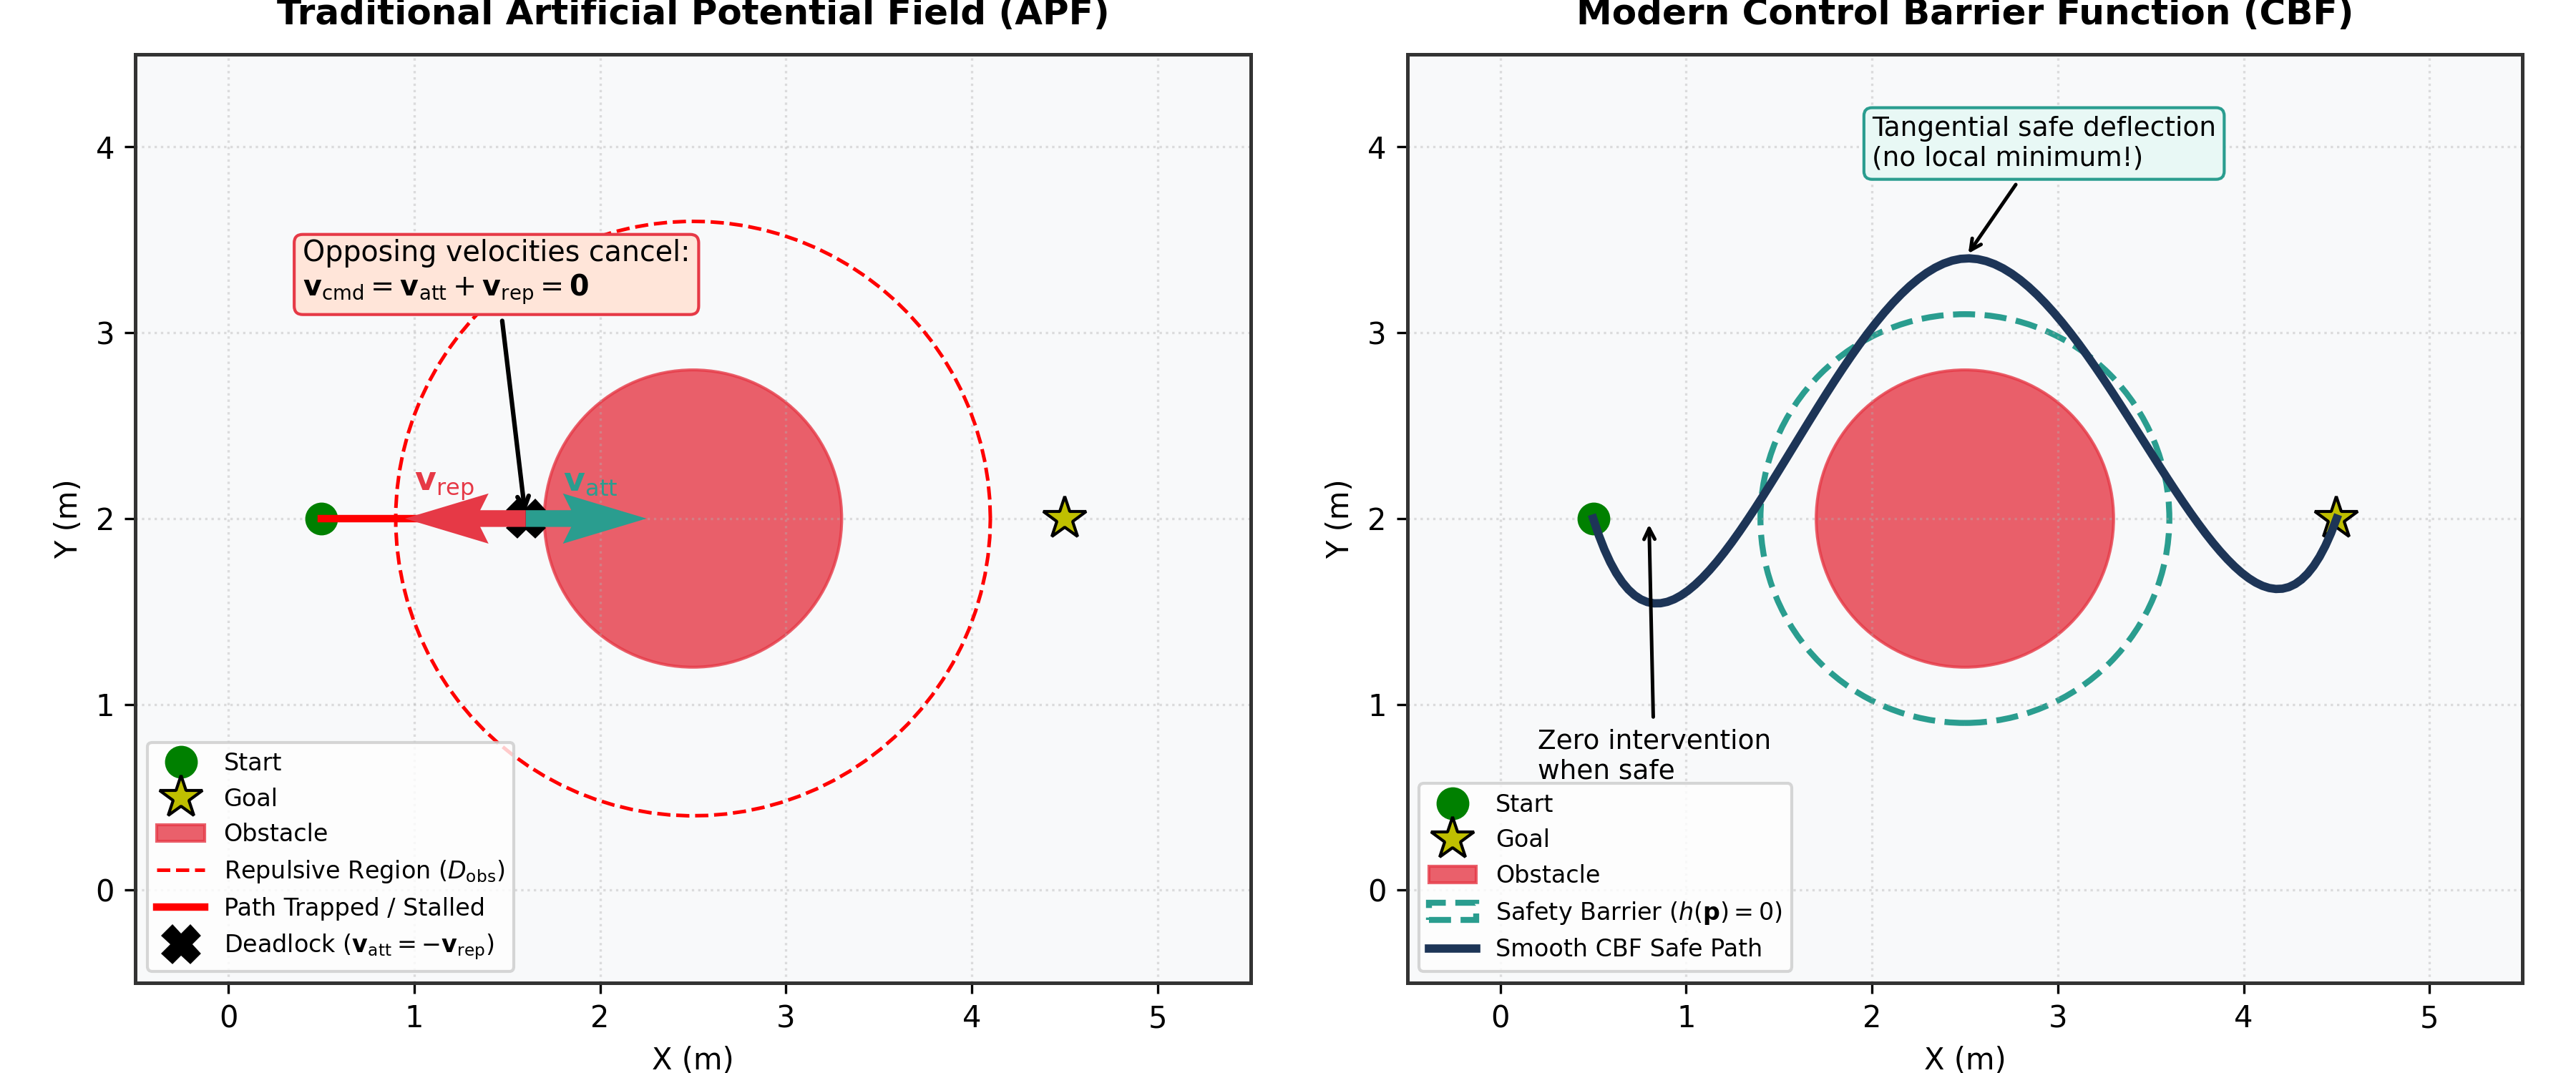
\includegraphics[width=\textwidth]{apf_vs_cbf_concept.png}
      \vspace{0.2em}
      \footnotesize \textbf{APF vs. CBF}: CBFs eliminate local minimum traps and enable smooth tangential circumnavigation.
      \footnotesize \textbf{Vector Cancellation}: At the local minimum, opposing velocities cancel out ($\mathbf{v}_{\mathrm{cmd}} = \mathbf{0}$).
    \end{column}
  \end{columns}
\end{frame}

% =============================================================================
% Slide 4: The CBF Philosophy: Minimal Intervention
% Slide 5: APF Failures 3 & 4 - Chattering & Parasitic Deflection
% =============================================================================
\begin{frame}{The CBF Philosophy: Safety as a Filter}
\begin{frame}{APF Failure Modes 3 \& 4: Chattering and Parasitic Deflection}
  \begin{center}
    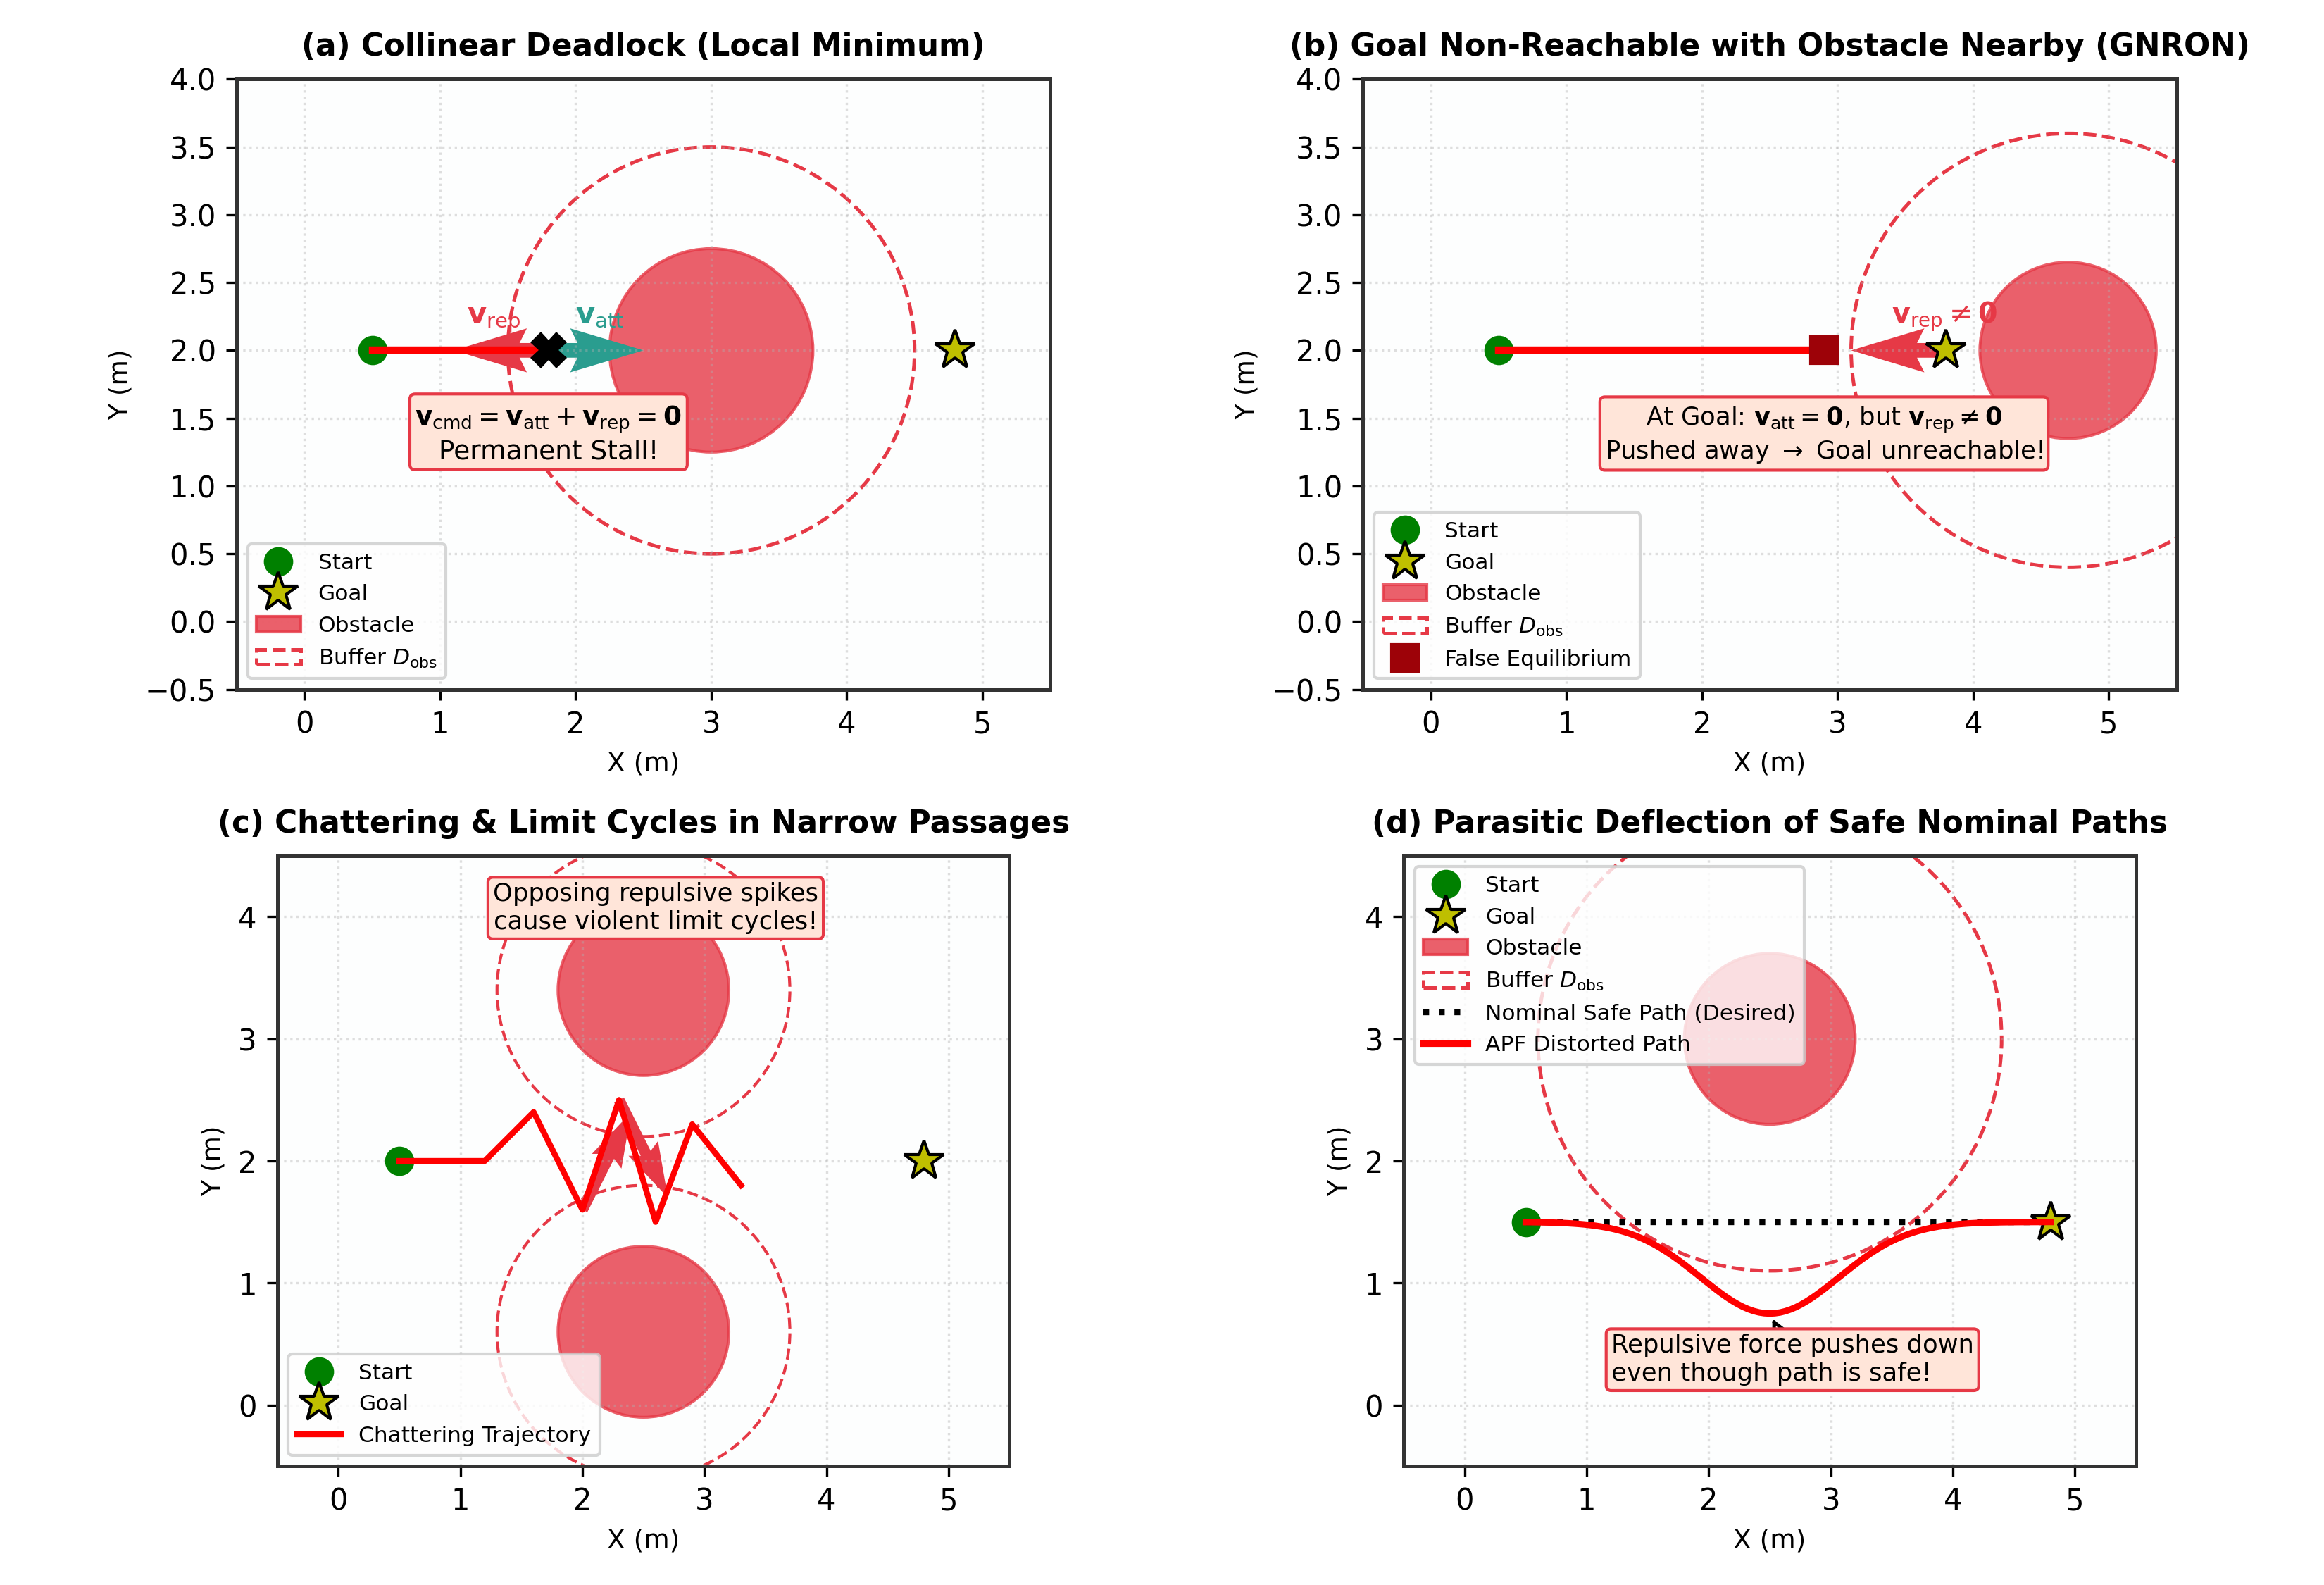
\includegraphics[height=0.55\textheight, keepaspectratio]{apf_failure_modes.png}
  \end{center}
  \vspace{-0.5em}
  \begin{columns}[T]
    \begin{column}{0.48\textwidth}
      \begin{block}{The Co-Pilot Analogy}
        Imagine a student learning to fly:
        \begin{itemize}
          \item The \textbf{student (PID)} holds the joystick and steers toward the waypoint.
          \item The \textbf{expert instructor (CBF)} sits quietly with hands off the controls.
          \item Only if the student is about to clip an obstacle does the instructor nudge the stick just enough to remain safe!
        \end{itemize}
      \end{block}
      \begin{alertblock}{Failure 3: Chattering in Narrow Corridors}
        \small Repulsion scales as $1/d^3$. Near walls, explosive velocity spikes cause the inner attitude loop to oscillate violently and destabilize.
      \end{alertblock}
    \end{column}

      \vspace{0.3em}
      \textbf{Key Concept: Forward Invariance}
      \begin{itemize}
        \item If you start in safe region $\mathcal{S}$, your control policy ensures you \textbf{never exit} $\mathcal{S}$ for all time $t \ge 0$.
      \end{itemize}
    \begin{column}{0.48\textwidth}
      \begin{alertblock}{Failure 4: Parasitic Path Distortion}
        \small APF pushes radially even when the drone is flying \textbf{parallel to} or \textbf{away from} the obstacle, distorting collision-free paths.
      \end{alertblock}
    \end{column}
  \end{columns}
\end{frame}

    \begin{column}{0.50\textwidth}
      \begin{exampleblock}{Core Benefits of CBF Safety Filters}
% =============================================================================
% Slide 6: The Paradigm Shift - Why CBF?
% =============================================================================
\begin{frame}{The Paradigm Shift: From Vector Sum to Safety Filter}
  \begin{columns}[T]
    \begin{column}{0.48\textwidth}
      \begin{block}{Why APF Breaks Down}
        \small
        APF attempts to solve two opposing goals simultaneously by \textbf{mixing them into one vector}:
        $$\mathbf{v} = \mathbf{v}_{\mathrm{att}} + \mathbf{v}_{\mathrm{rep}}$$
        This force fight corrupts nominal tracking and creates spurious zero-velocity equilibria.
      \end{block}

      \vspace{0.1em}
      \begin{exampleblock}{The CBF Solution: Decoupling}
        \scriptsize
        \begin{enumerate}
          \item \textbf{Minimally Invasive}: If trajectory is safe, CBF does \textit{nothing} ($\mathbf{v}^* = \mathbf{v}_{\mathrm{des}}$).
          \item \textbf{Guaranteed Safety}: Provable set forward-invariance under continuous dynamics.
          \item \textbf{Decoupled Design}: Change goal planner freely without modifying safety logic!
          \item \textbf{Goal Tracker}: Computes nominal velocity $\mathbf{v}_{\mathrm{des}}$.
          \item \textbf{Safety Filter}: Defines safe velocity set $\mathcal{K}(\mathbf{p})$.
          \item \textbf{Minimal Intervention}: Projects $\mathbf{v}_{\mathrm{des}} \to \mathbf{v}^*$ only when danger is imminent!
        \end{enumerate}
      \end{exampleblock}
    \end{column}

    \begin{column}{0.50\textwidth}
      \begin{block}{The Co-Pilot Analogy}
        \small
        \begin{itemize}
          \item The \textbf{student (PID)} steers toward the waypoint.
          \item The \textbf{instructor (CBF Filter)} sits quietly with hands off the controls.
          \item If and only if the student is about to clip an obstacle does the instructor nudge the stick just enough to remain safe!
        \end{itemize}
      \end{block}

      \vspace{0.3em}
      \centering
      \small \textbf{Nominal Intent} $\xrightarrow{\text{PID}}$ $\mathbf{v}_{\mathrm{des}}$ $\xrightarrow[\textbf{CBF Safety Filter}]{\text{Shield}}$ $\mathbf{v}^*$ $\xrightarrow{\text{Attitude}}$ $\mathbf{u}_{\mathrm{motors}}$
      \small \textbf{Nominal Velocity} $\mathbf{v}_{\mathrm{des}}$ $\xrightarrow[\textbf{CBF Filter}]{\text{Shield}}$ $\mathbf{v}^*$ $\xrightarrow{\text{Attitude Loop}}$ Motor Thrusts
    \end{column}
  \end{columns}
\end{frame}

% =============================================================================
% Slide 5: Step 1 - Quantifying Safety with h(p)
% Slide 7: Step 1 - Quantifying Safety with h(p)
% =============================================================================
\begin{frame}{Step 1: Quantifying Safety with Barrier Function $h(\mathbf{p})$}
  \begin{columns}[T]
    \begin{column}{0.54\textwidth}
      For a spherical obstacle at position $\mathbf{p}_{\mathrm{obs}}$ with safety buffer $D_{\mathrm{obs}}$:
      \begin{equation*}
        h(\mathbf{p}) = \|\mathbf{p} - \mathbf{p}_{\mathrm{obs}}\| - D_{\mathrm{obs}}
      \end{equation*}

      \begin{block}{Three Fundamental Topological Zones}
      \begin{block}{Three Fundamental Topological Sets}
        \small
        \begin{itemize}
          \item \textbf{Safe Zone ($\mathcal{S}$)}: $h(\mathbf{p}) > 0$ (outside safety buffer)
          \item \textbf{Safe Set ($\mathcal{S}$)}: $h(\mathbf{p}) \ge 0$ (outside safety buffer)
          \item \textbf{Safety Boundary ($\partial \mathcal{S}$)}: $h(\mathbf{p}) = 0$ (contact boundary)
          \item \textbf{Danger Zone (Unsafe)}: $h(\mathbf{p}) < 0$ (buffer penetrated!)
          \item \textbf{Unsafe Set}: $h(\mathbf{p}) < 0$ (buffer penetrated!)
        \end{itemize}
      \end{block}

      \vspace{0.3em}
      \vspace{0.2em}
      \textbf{Outward Normal Vector (Gradient)}:
      $$\nabla h(\mathbf{p}) = \frac{\mathbf{p} - \mathbf{p}_{\mathrm{obs}}}{\|\mathbf{p} - \mathbf{p}_{\mathrm{obs}}\|}, \qquad \|\nabla h(\mathbf{p})\| = 1$$
    \end{column}

    \begin{column}{0.44\textwidth}
      \centering
      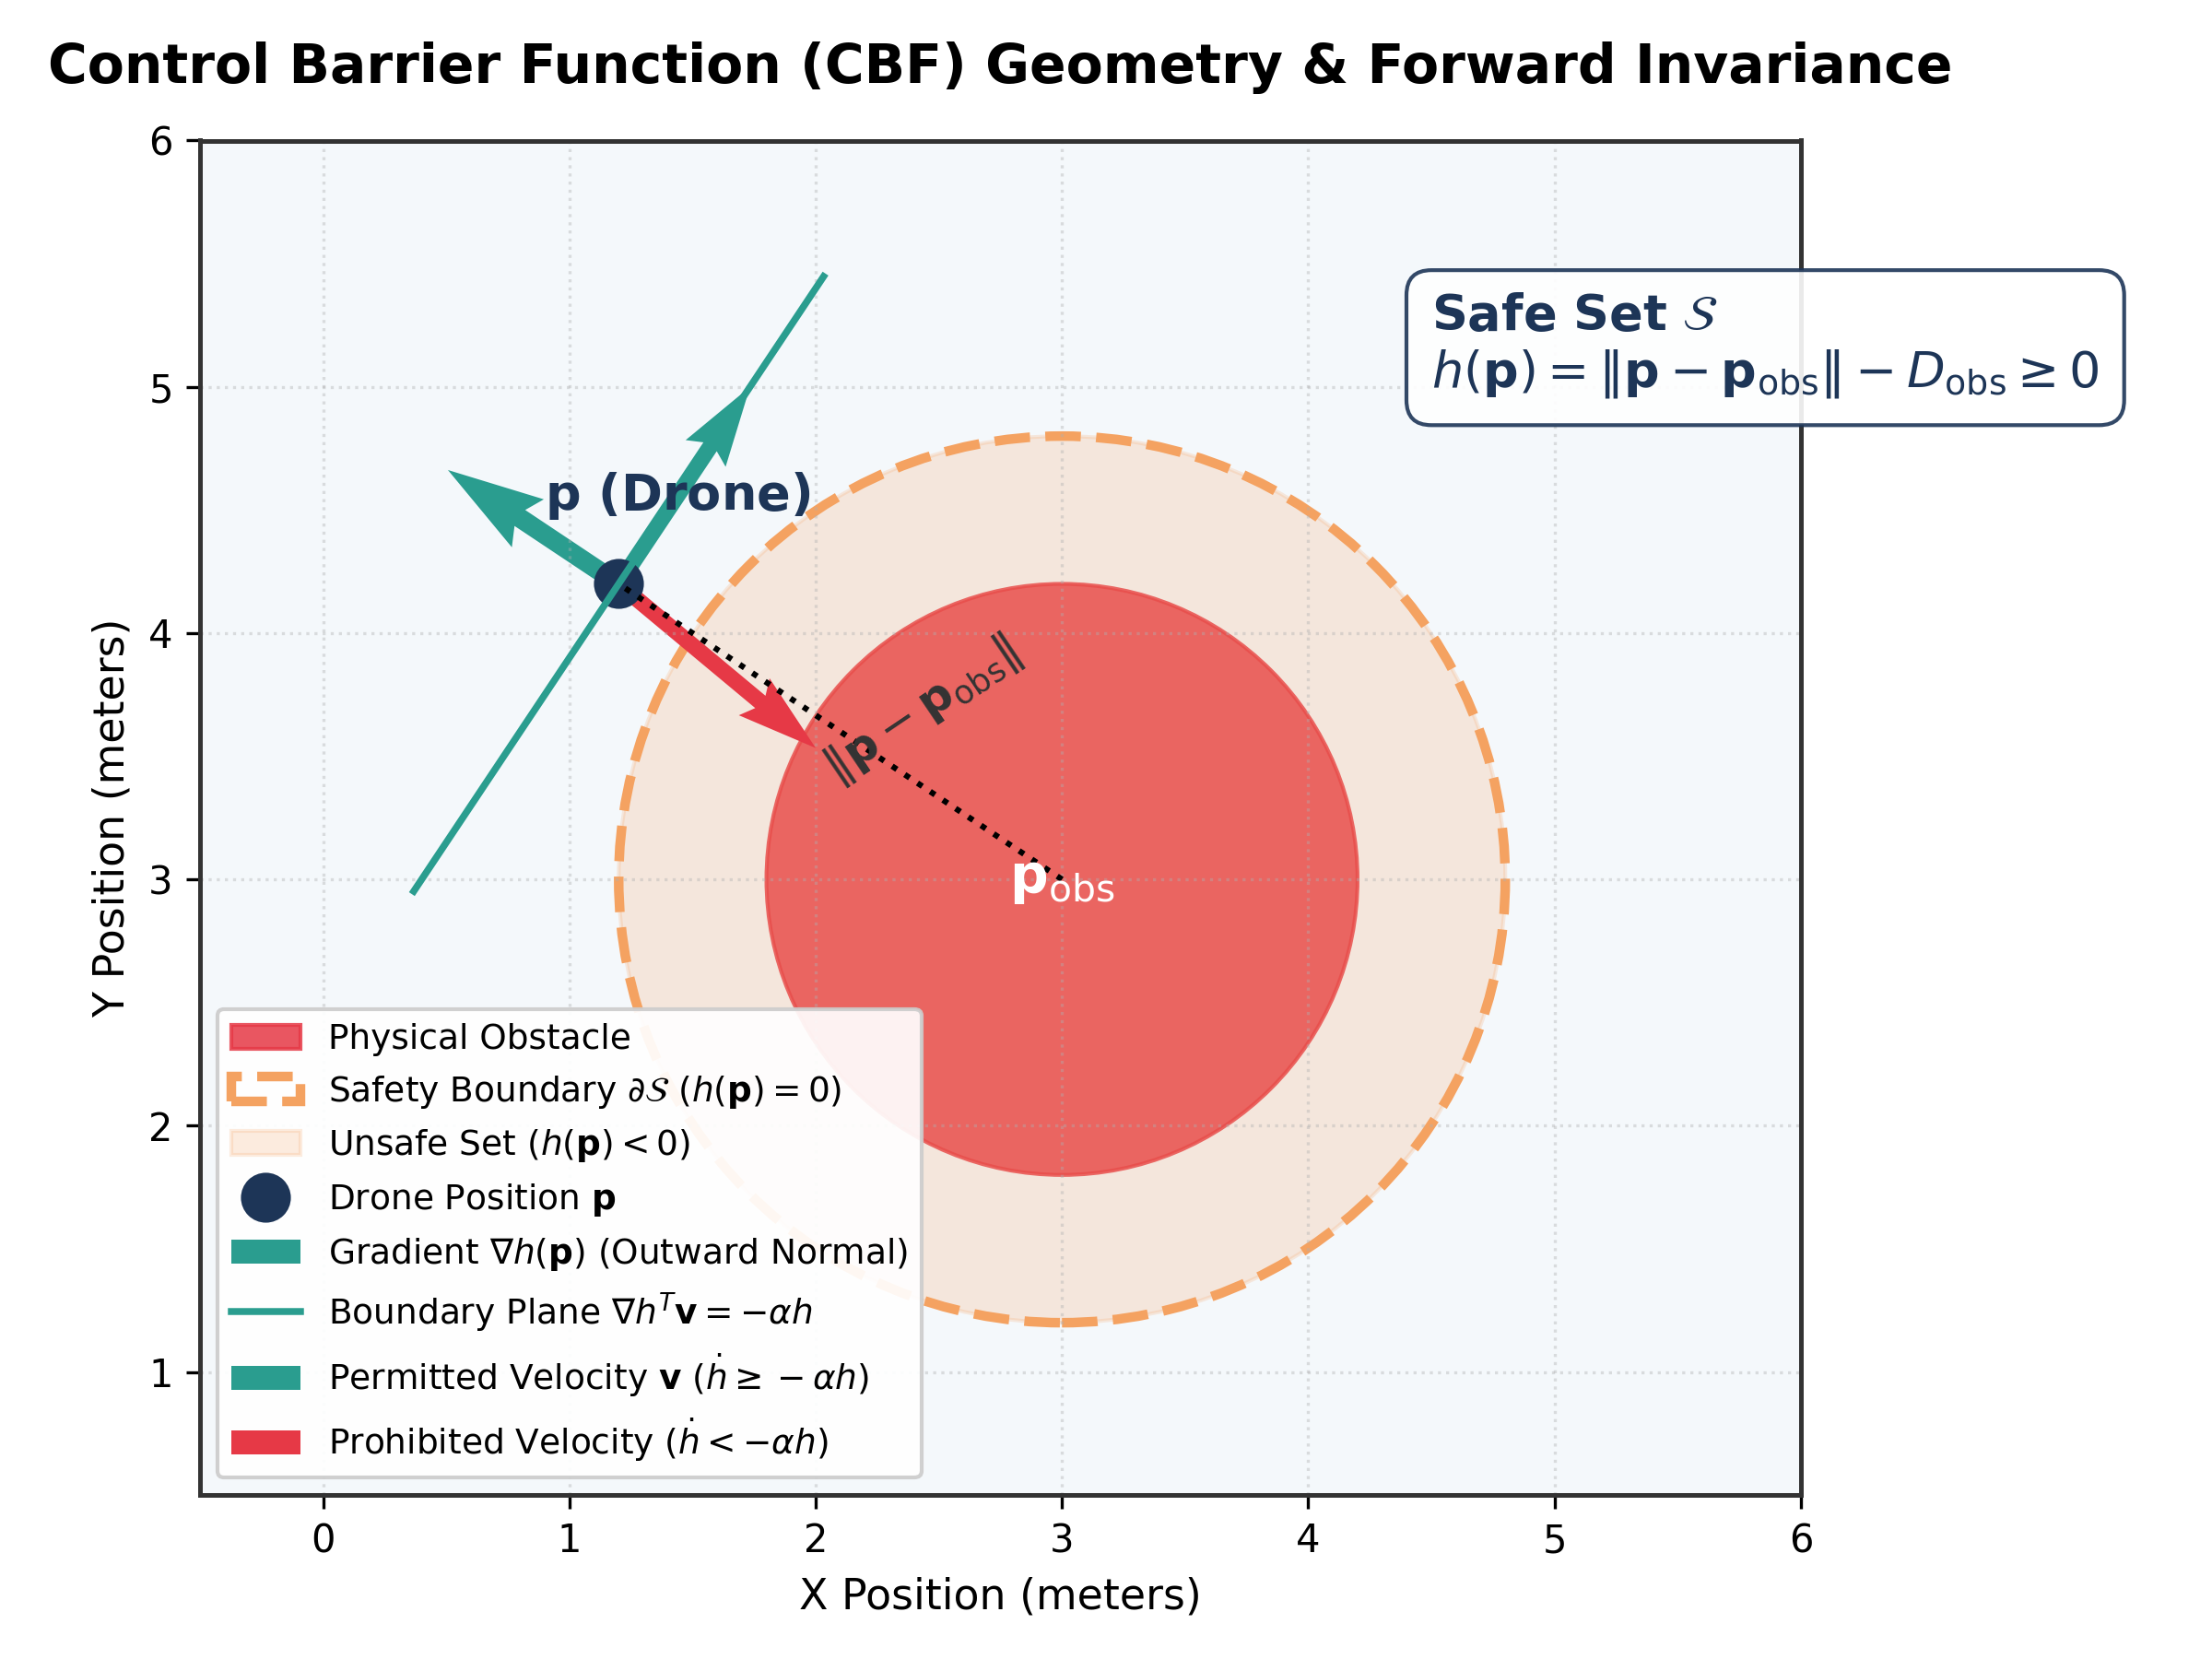
\includegraphics[width=\textwidth]{cbf_concept_diagram.png}
      \vspace{0.2em}
      \footnotesize Outward gradient $\nabla h(\mathbf{p})$ defines the forbidden and permitted velocity half-spaces.
      \footnotesize Outward gradient $\nabla h(\mathbf{p})$ defines the barrier boundary and permitted velocity half-space.
    \end{column}
  \end{columns}
\end{frame}

% =============================================================================
% Slide 6: Step 2 - The Barrier Velocity Condition
% Slide 8: Step 2 - The Barrier Velocity Condition
% =============================================================================
\begin{frame}{Step 2: The Barrier Condition: $\dot{h} \ge -\alpha h$}
\begin{frame}{Step 2: The Barrier Condition: $\dot{h} \ge -\alpha h(\mathbf{p})$}
  \begin{columns}[T]
    \begin{column}{0.53\textwidth}
      How does safety change as the drone moves with velocity $\mathbf{v} = \mathbf{\dot{p}}$?
      How does safety margin change as the drone moves with velocity $\mathbf{v} = \mathbf{\dot{p}}$?
      $$\dot{h}(\mathbf{p}, \mathbf{v}) = \nabla h(\mathbf{p})^T \mathbf{v}$$

      \begin{block}{The Control Barrier Inequality (Ames et al.)}
        $$\dot{h}(\mathbf{p}, \mathbf{v}) \ge -\alpha h(\mathbf{p}) \iff \nabla h(\mathbf{p})^T \mathbf{v} \ge -\alpha h(\mathbf{p})$$
      \end{block}

      \small
      \textbf{Physical Meaning (Dynamic Speed Limit)}:
      \begin{itemize}
        \item \textbf{Far away} ($h \gg 0$): Can fly toward obstacle fast.
        \item \textbf{Approaching} ($h \to 0$): Inward speed throttled.
        \item \textbf{At boundary} ($h = 0$): Inward motion forbidden ($\nabla h^T \mathbf{v} \ge 0$).
        \item \textbf{Far away} ($h \gg 0$): Allowed to fly toward obstacle fast.
        \item \textbf{Approaching} ($h \to 0$): Inward speed smoothly throttled.
        \item \textbf{At boundary} ($h = 0$): Inward motion strictly forbidden ($\nabla h^T \mathbf{v} \ge 0$).
      \end{itemize}
    \end{column}

    \begin{column}{0.45\textwidth}
      \begin{exampleblock}{Everyday Analogy: Smooth Braking}
        \small
        \begin{itemize}
          \item Bad drivers slam brakes at the last second.
          \item Smooth drivers brake gradually: speed limit is proportional to distance remaining!
          \item A bad driver slams brakes at the last second.
          \item A smooth driver brakes gradually: speed limit is proportional to distance remaining!
          \item That is exactly what $\dot{h} \ge -\alpha h$ enforces.
        \end{itemize}
      \end{exampleblock}

      \vspace{0.2em}
      \begin{alertblock}{Tuning $\alpha$ (Class-$\mathcal{K}$ Gain)}
        \small
        \begin{itemize}
          \item \textbf{Small $\alpha$ (0.5)}: Early, gentle, conservative.
          \item \textbf{Large $\alpha$ (2.5)}: Tighter, aggressive, fast.
          \item \textbf{Large $\alpha$ (2.5)}: Tighter, agile, aggressive turn.
        \end{itemize}
      \end{alertblock}
    \end{column}
  \end{columns}
\end{frame}

% =============================================================================
% Slide 7: The Safety Filter (CBF-QP) Formulation
% Slide 9: Exact Closed-Form Solution for Single Integrators
% =============================================================================
\begin{frame}{The CBF Quadratic Program (CBF-QP) Safety Filter}
\begin{frame}{The CBF-QP Safety Filter: Exact Closed-Form Solution}
  \begin{columns}[T]
    \begin{column}{0.52\textwidth}
      We formulate safety filtering as an instantaneous \textbf{Quadratic Program (QP)}:

      \begin{block}{The Optimization Problem}
        \begin{align*}
          \mathbf{v}^* = \arg\min_{\mathbf{v} \in \mathbb{R}^3} \quad & \frac{1}{2} \|\mathbf{v} - \mathbf{v}_{\mathrm{des}}\|^2 \\
          \text{subject to} \quad & \nabla h(\mathbf{p})^T \mathbf{v} \ge -\alpha h(\mathbf{p})
        \end{align*}
      \end{block}

      \textbf{What this means in plain English}:
      \begin{itemize}
        \item \textbf{Objective}: Stay as close as humanly possible to desired flight command $\mathbf{v}_{\mathrm{des}}$.
        \item \textbf{Constraint}: Obey the linear barrier inequality.
      \end{itemize}
    \end{column}

    \begin{column}{0.46\textwidth}
      \begin{exampleblock}{Two Operating Regimes}
        \textbf{Case 1: Safe Trajectory}
        \begin{itemize}
          \item If $\nabla h^T \mathbf{v}_{\mathrm{des}} \ge -\alpha h$:
          \item $\mathbf{v}^* = \mathbf{v}_{\mathrm{des}}$ (Zero intervention!)
        \end{itemize}
        \vspace{0.3em}
        \textbf{Case 2: Dangerous Trajectory}
        \begin{itemize}
          \item If $\nabla h^T \mathbf{v}_{\mathrm{des}} < -\alpha h$:
          \item Project $\mathbf{v}_{\mathrm{des}}$ onto boundary of safe half-space!
        \end{itemize}
      \end{exampleblock}

      \vspace{0.3em}
      \small \textbf{Key Question}: Do we need a heavy, slow QP solver on an embedded flight MCU?
      \textbf{Answer}: \textbf{NO!}
    \end{column}
  \end{columns}
\end{frame}

% =============================================================================
% Slide 8: Exact Closed-Form Solution
% =============================================================================
\begin{frame}{Exact Closed-Form Solution for Single Integrators}
  \begin{columns}[T]
    \begin{column}{0.54\textwidth}
      Because $\|\nabla h(\mathbf{p})\| = 1$, the Karush-Kuhn-Tucker (KKT) conditions yield an \textbf{analytical closed-form solution}!
      We formulate safety filtering as a Quadratic Program:
      $$\mathbf{v}^* = \arg\min_{\mathbf{v} \in \mathbb{R}^3} \frac{1}{2}\|\mathbf{v} - \mathbf{v}_{\mathrm{des}}\|^2 \quad \text{s.t.} \quad \nabla h^T \mathbf{v} \ge -\alpha h$$

      \begin{block}{The Closed-Form Formula}
      \begin{block}{Analytical KKT Solution}
        \small
        Define the safety violation scalar $\Psi$:
        \begin{equation*}
          \Psi = \nabla h(\mathbf{p})^T \mathbf{v}_{\mathrm{des}} + \alpha h(\mathbf{p})
        \end{equation*}
        $$\Psi = \nabla h(\mathbf{p})^T \mathbf{v}_{\mathrm{des}} + \alpha h(\mathbf{p})$$
        \begin{itemize}
          \item If $\Psi \ge 0$: $\mathbf{v}^* = \mathbf{v}_{\mathrm{des}}$ (Nominal is safe)
          \item If $\Psi \ge 0$: $\mathbf{v}^* = \mathbf{v}_{\mathrm{des}}$ \textbf{(Zero intervention!)}
          \item If $\Psi < 0$: $\mathbf{v}^* = \mathbf{v}_{\mathrm{des}} - \Psi \nabla h(\mathbf{p})$
        \end{itemize}
      \end{block}

      \small
      \scriptsize
      \begin{itemize}
        \item One dot product + one vector subtraction ($< 1\,\mu\text{s}$)!
        \item No numerical solver required onboard.
        \item Guaranteed minimal Euclidean deviation $\|\mathbf{v}^* - \mathbf{v}_{\mathrm{des}}\|$.
        \item One dot product + vector subtraction ($< 1\,\mu\text{s}$)!
        \item No numerical QP solver needed on flight MCU.
        \item Guaranteed minimal distortion $\|\mathbf{v}^* - \mathbf{v}_{\mathrm{des}}\|$.
      \end{itemize}
    \end{column}

    \begin{column}{0.44\textwidth}
      \centering
      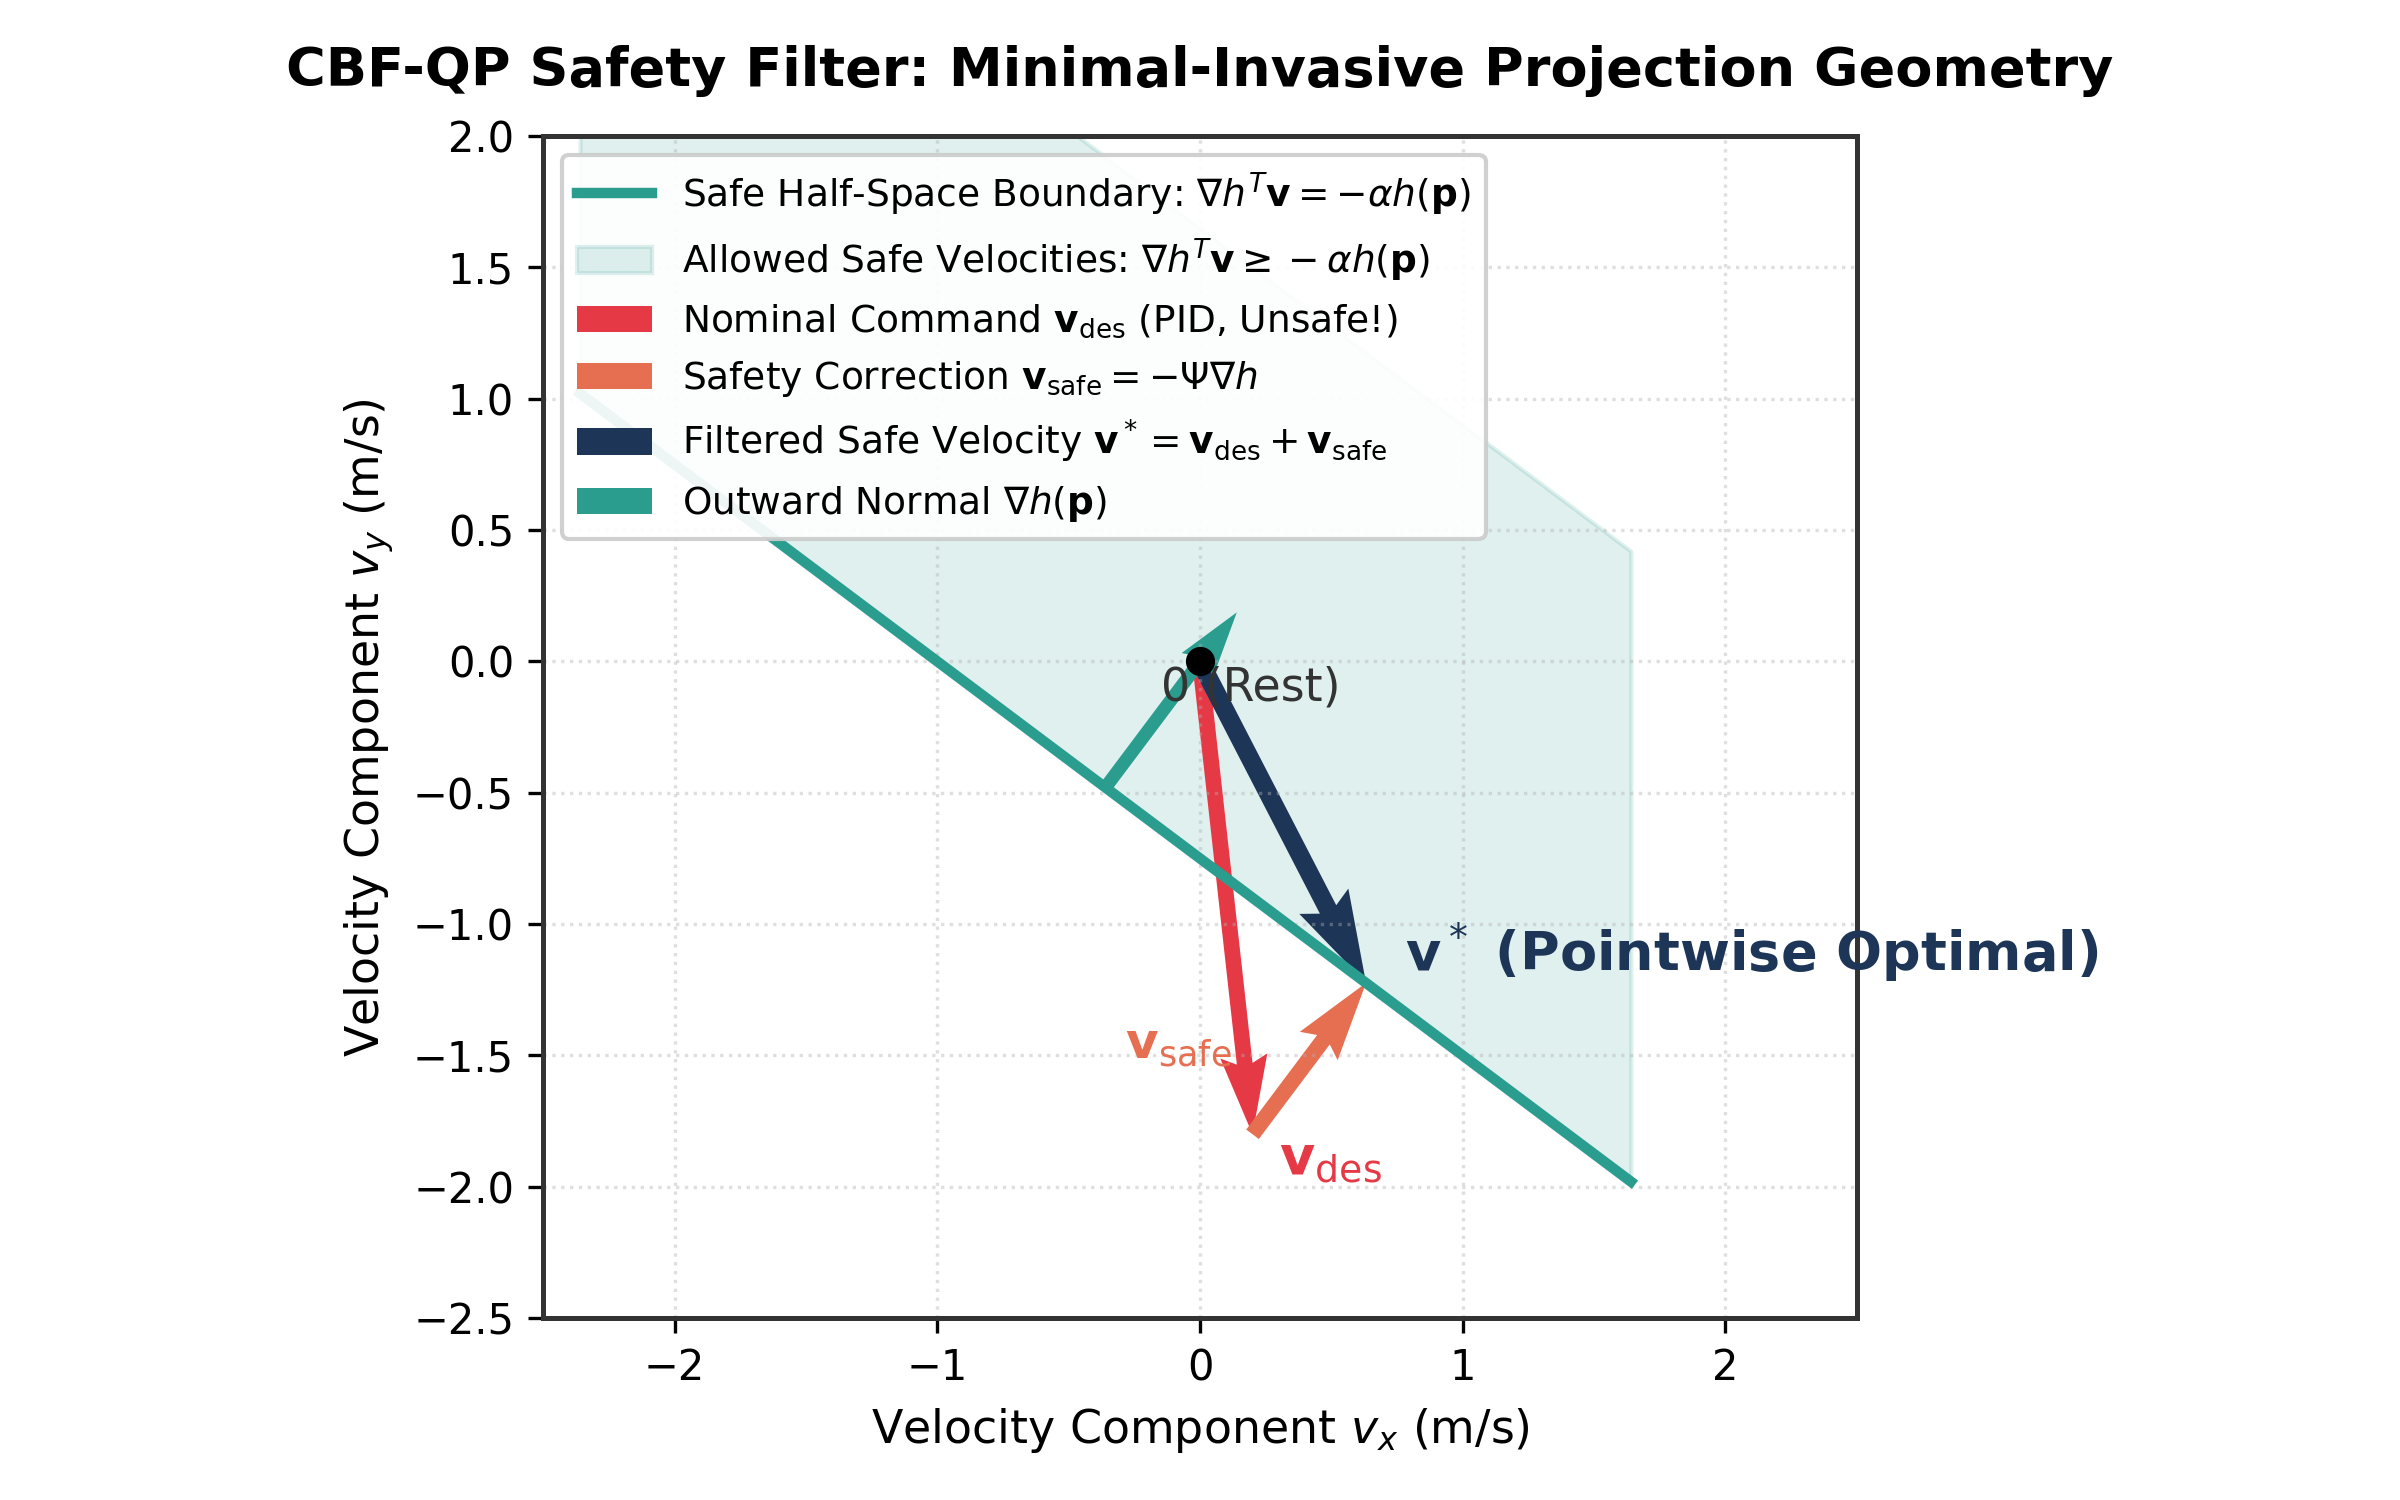
\includegraphics[width=\textwidth]{cbf_projection_geometry.png}
      \vspace{0.2em}
      \footnotesize \textbf{Geometric Projection}: When $\Psi < 0$, $\mathbf{v}_{\mathrm{des}}$ is projected orthogonally along $\nabla h$ onto the safe boundary.
    \end{column}
  \end{columns}
\end{frame}

% =============================================================================
% Slide 9: Hierarchical 6-DOF Quadrotor Architecture
% Slide 10: How CBF Solves All Four APF Failures
% =============================================================================
\begin{frame}{Hierarchical Quadrotor Architecture}
  \centering
  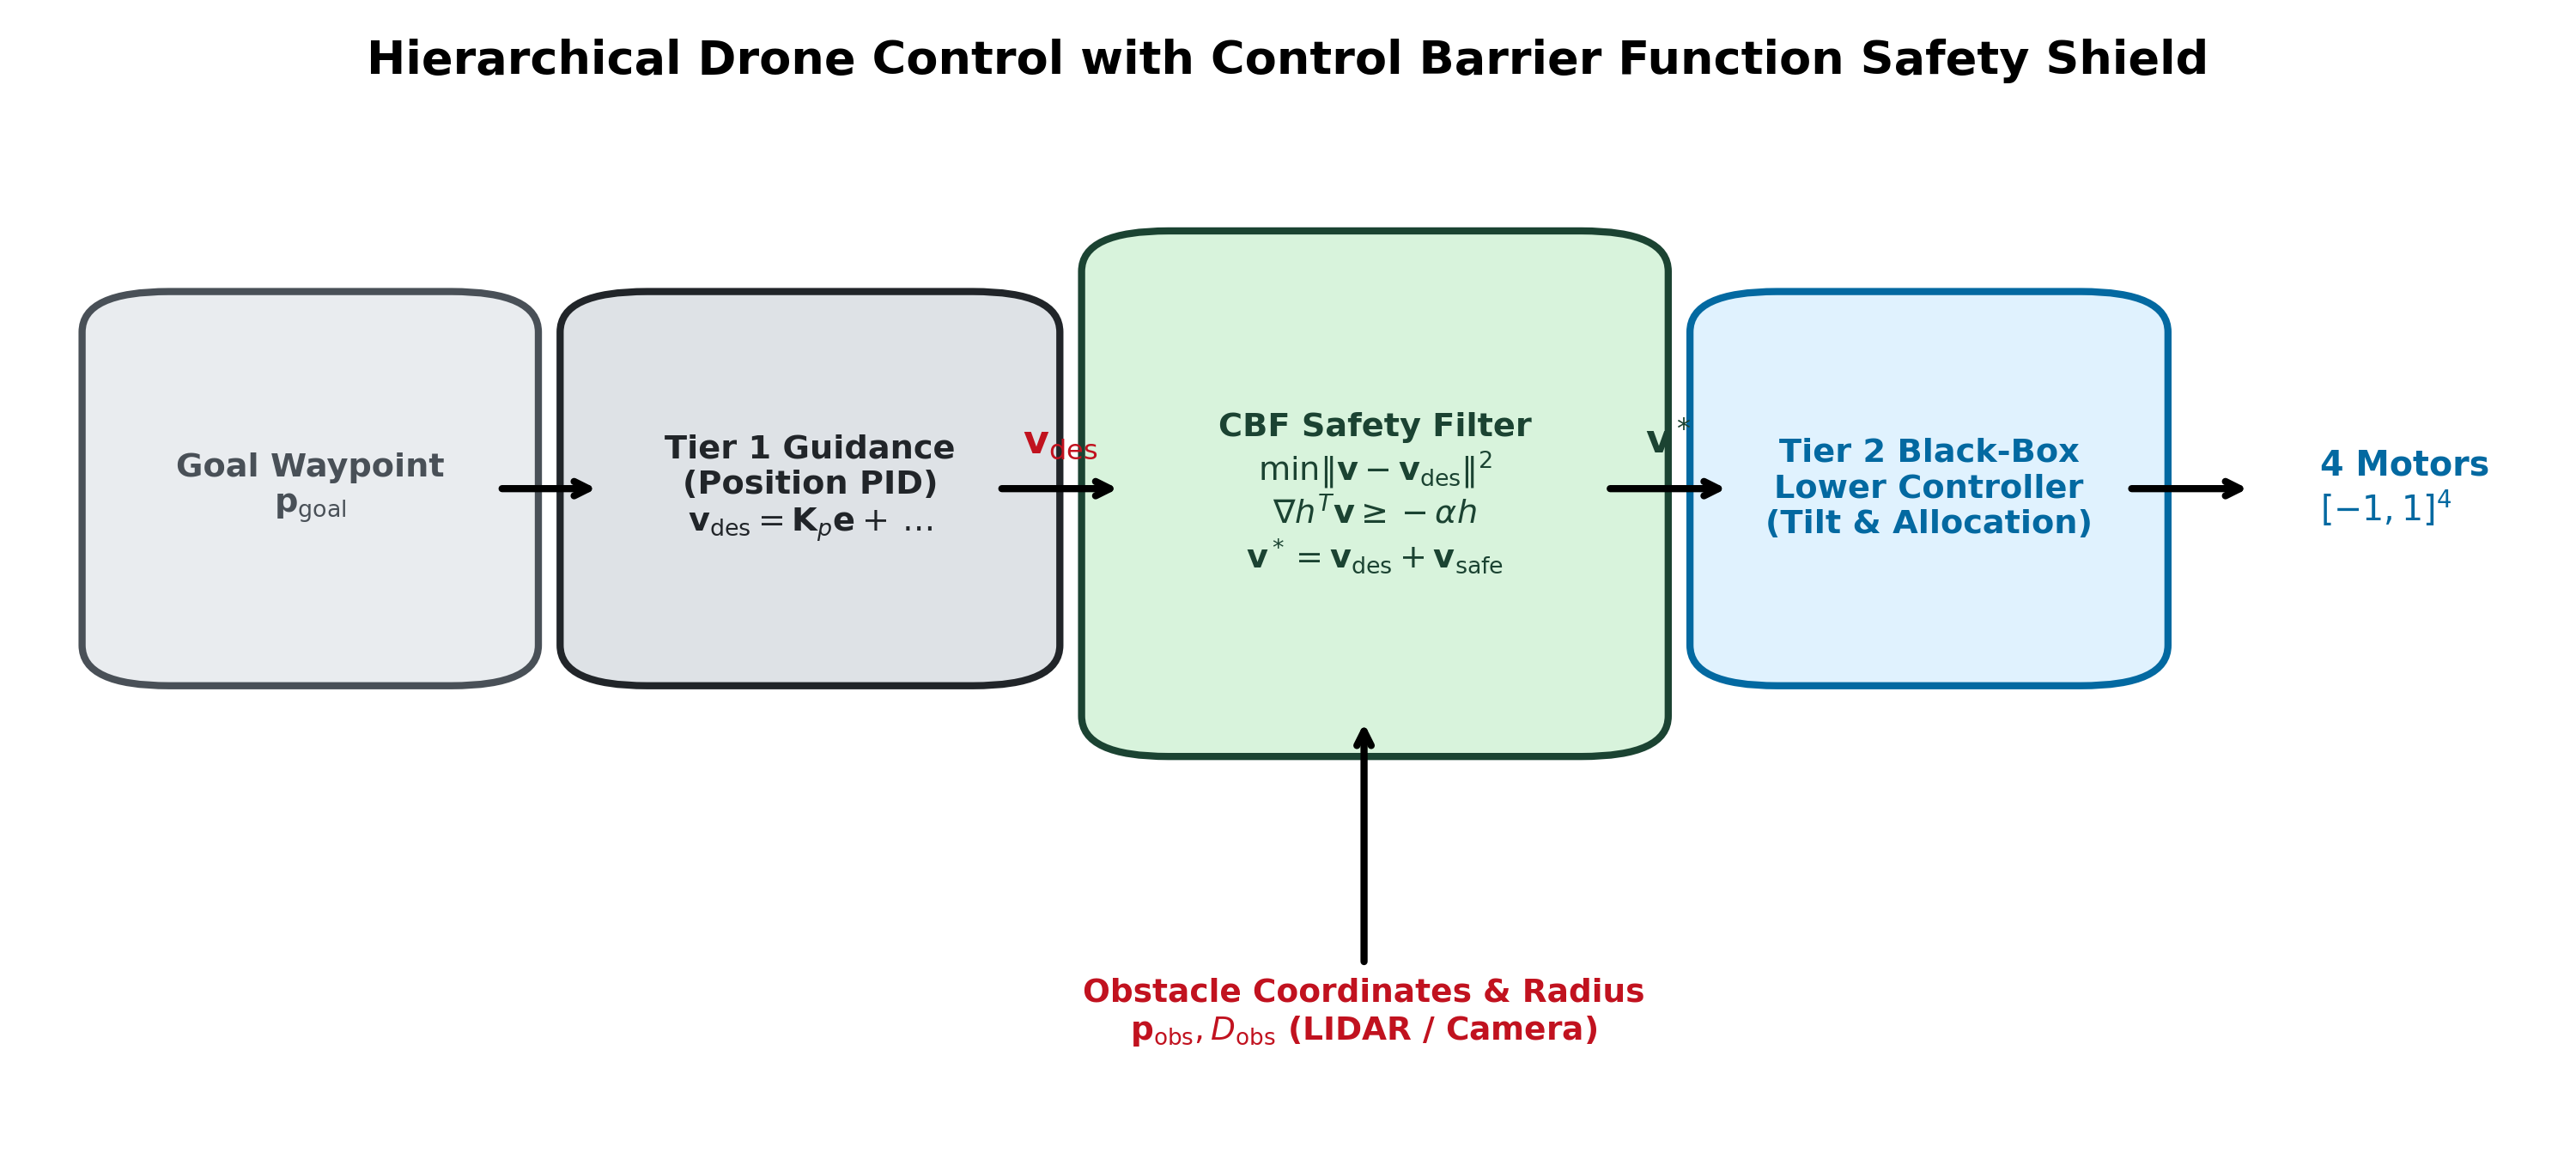
\includegraphics[height=0.34\textheight, keepaspectratio]{cbf_architecture_block.png}

  \vspace{0.2em}
\begin{frame}{Why CBFs Overcome All Four APF Failure Modes}
  \begin{columns}[T]
    \begin{column}{0.48\textwidth}
      \begin{block}{Tier 1: High-Level Guidance \& Safety}
      \begin{exampleblock}{1. No Collinear Deadlocks (Traps)}
        \small
        \begin{itemize}
          \item Kinematic model: $\mathbf{\dot{p}} = \mathbf{v}_{\mathrm{cmd}}$
          \item Goal PID computes nominal velocity $\mathbf{v}_{\mathrm{des}}$
          \item \textbf{CBF Safety Filter} converts $\mathbf{v}_{\mathrm{des}} \to \mathbf{v}^*$
          \item APF: Opposing velocities cancel out ($\mathbf{v} = \mathbf{0}$).
          \item \textbf{CBF}: Only normal inward component restricted. Tangential plane is \textbf{unconstrained} $\implies$ smooth slide!
        \end{itemize}
      \end{block}
    \end{column}
      \end{exampleblock}

    \begin{column}{0.48\textwidth}
      \begin{block}{Tier 2: Low-Level 6-DOF Dynamics}
      \begin{exampleblock}{2. No GNRON (Goal Near Obstacle)}
        \small
        \begin{itemize}
          \item Inner-loop tracking: Black-box attitude PID
          \item Tilts drone (pitch $\theta$, roll $\phi$) to achieve $\mathbf{v}^*$
          \item Allocates 4 motor thrusts $\Omega_{1,2,3,4} \in [-1, 1]^4$
          \item APF: $\mathbf{v}_{\mathrm{rep}} \ne \mathbf{0}$ at goal pushes drone away.
          \item \textbf{CBF}: As $\mathbf{p} \to \mathbf{p}_{\mathrm{goal}}$, $\mathbf{v}_{\mathrm{des}} \to \mathbf{0} \implies \nabla h^T \mathbf{0} \ge -\alpha h$. Drone stops exactly at the goal!
        \end{itemize}
      \end{block}
      \end{exampleblock}
    \end{column}
  \end{columns}
\end{frame}

% =============================================================================
% Slide 10: MuJoCo Simulation Experiment Setup
% =============================================================================
\begin{frame}{MuJoCo Simulation Benchmark: The Collision Course}
  \begin{columns}[T]
    \begin{column}{0.50\textwidth}
      \textbf{Flight Arena Parameters}:
      \begin{itemize}
        \item Initial Drone Hover: $[0.0, 0.0, 0.5]\,\text{m}$
        \item Target Goal Waypoint: $[1.2, 1.2, 1.6]\,\text{m}$
        \item Straight-line path length: $2.10\,\text{m}$
      \end{itemize}

      \vspace{0.3em}
      \textbf{Spherical Obstacle}:
      \begin{itemize}
        \item Position: $\mathbf{p}_{\mathrm{obs}} = [0.6, 0.6, 1.05]\,\text{m}$ (directly in center!)
        \item Obstacle Physical Radius: $R_{\mathrm{obs}} = 0.22\,\text{m}$
        \item Quadrotor Blade Tip Radius: $R_{\mathrm{drone}} = 0.17\,\text{m}$
        \item Physical collision limit: $R_{\mathrm{crit}} = 0.39\,\text{m}$
        \item Configured Safety Buffer: $D_{\mathrm{obs}} = 0.55\,\text{m}$, $\alpha = 2.2$
      \end{itemize}
    \end{column}

    \begin{column}{0.48\textwidth}
      \begin{alertblock}{Experiment A: Unfiltered PID Baseline}
      \begin{exampleblock}{3. No Chattering / Limit Cycles}
        \small
        \begin{itemize}
          \item Nominal PID runs without CBF shield.
          \item Steers straight down the line of sight.
          \item APF: $1/d^3$ gradient explosion triggers attitude oscillations.
          \item \textbf{CBF}: Linear velocity constraint produces smooth, bounded deflections.
        \end{itemize}
      \end{alertblock}
      \end{exampleblock}

      \vspace{0.4em}
      \begin{exampleblock}{Experiment B: With CBF Safety Shield}
      \begin{exampleblock}{4. Zero Parasitic Deflection}
        \small
        \begin{itemize}
          \item Exact same goal PID gains.
          \item Closed-form single-integrator CBF filter active.
          \item APF: Repels even when flying parallel/away.
          \item \textbf{CBF}: Flying parallel or away satisfies $\Psi \ge 0 \implies \mathbf{v}^* = \mathbf{v}_{\mathrm{des}}$ (100\% unhampered tracking!).
        \end{itemize}
      \end{exampleblock}
    \end{column}
  \end{columns}
\end{frame}

% =============================================================================
% Slide 11: MuJoCo 6-DOF Simulation Results
% Slide 11: Head-to-Head Comparison Table
% =============================================================================
\begin{frame}{Flight Verification: Unfiltered vs. CBF Filtered}
\begin{frame}{Head-to-Head Analytical Comparison: APF vs. CBF}
  \centering
  \resizebox{\textwidth}{!}{%
  \begin{tabular}{lcc}
    \toprule
    \textbf{Feature} & \textbf{Artificial Potential Fields (APF)} & \textbf{Control Barrier Functions (CBF)} \\
    \midrule
    \textbf{Core Paradigm} & Vector Sum: $\mathbf{v}_{\mathrm{att}} + \mathbf{v}_{\mathrm{rep}}$ & Constrained Projection: $\arg\min \|\mathbf{v} - \mathbf{v}_{\mathrm{des}}\|^2$ \\
    \textbf{Safety Formulation} & Soft energy penalty $U_{\mathrm{rep}}$ & Hard forward-invariance set constraint \\
    \textbf{Nominal Preservation} & Corrupted inside $D_{\mathrm{obs}}$ & \textbf{Preserved exactly} whenever safe ($\mathbf{v}^* = \mathbf{v}_{\mathrm{des}}$) \\
    \textbf{Collinear Deadlock} & \textcolor{AlertRed}{\textbf{Severe (permanent stall)}} & \textcolor{SafeGreen}{\textbf{Eliminated (tangential slide)}} \\
    \textbf{Goal Near Obstacle} & \textcolor{AlertRed}{\textbf{Fails (equilibrium shifted)}} & \textcolor{SafeGreen}{\textbf{Guaranteed exact arrival}} \\
    \textbf{Chattering Oscillations} & High ($1/d^3$ explosive gradient) & \textcolor{SafeGreen}{\textbf{None (smooth linear boundary)}} \\
    \textbf{Computational Cost} & $\mathcal{O}(1)$ vector sum & $\mathcal{O}(1)$ closed-form KKT formula \\
    \textbf{Formal Guarantees} & None & \textbf{Provable forward invariance} $\mathbf{p}(t) \in \mathcal{S}$ \\
    \bottomrule
  \end{tabular}%
  }

  \vspace{0.3em}
  \begin{block}{Summary Takeaway}
    \small CBF retains the analytical speed of APF ($\mathcal{O}(1)$ closed-form) while eliminating all topological traps and providing formal set-invariance safety guarantees!
  \end{block}
\end{frame}

% =============================================================================
% Slide 12: MuJoCo Simulation Results
% =============================================================================
\begin{frame}{Flight Verification in 6-DOF MuJoCo Simulation}
  \centering
  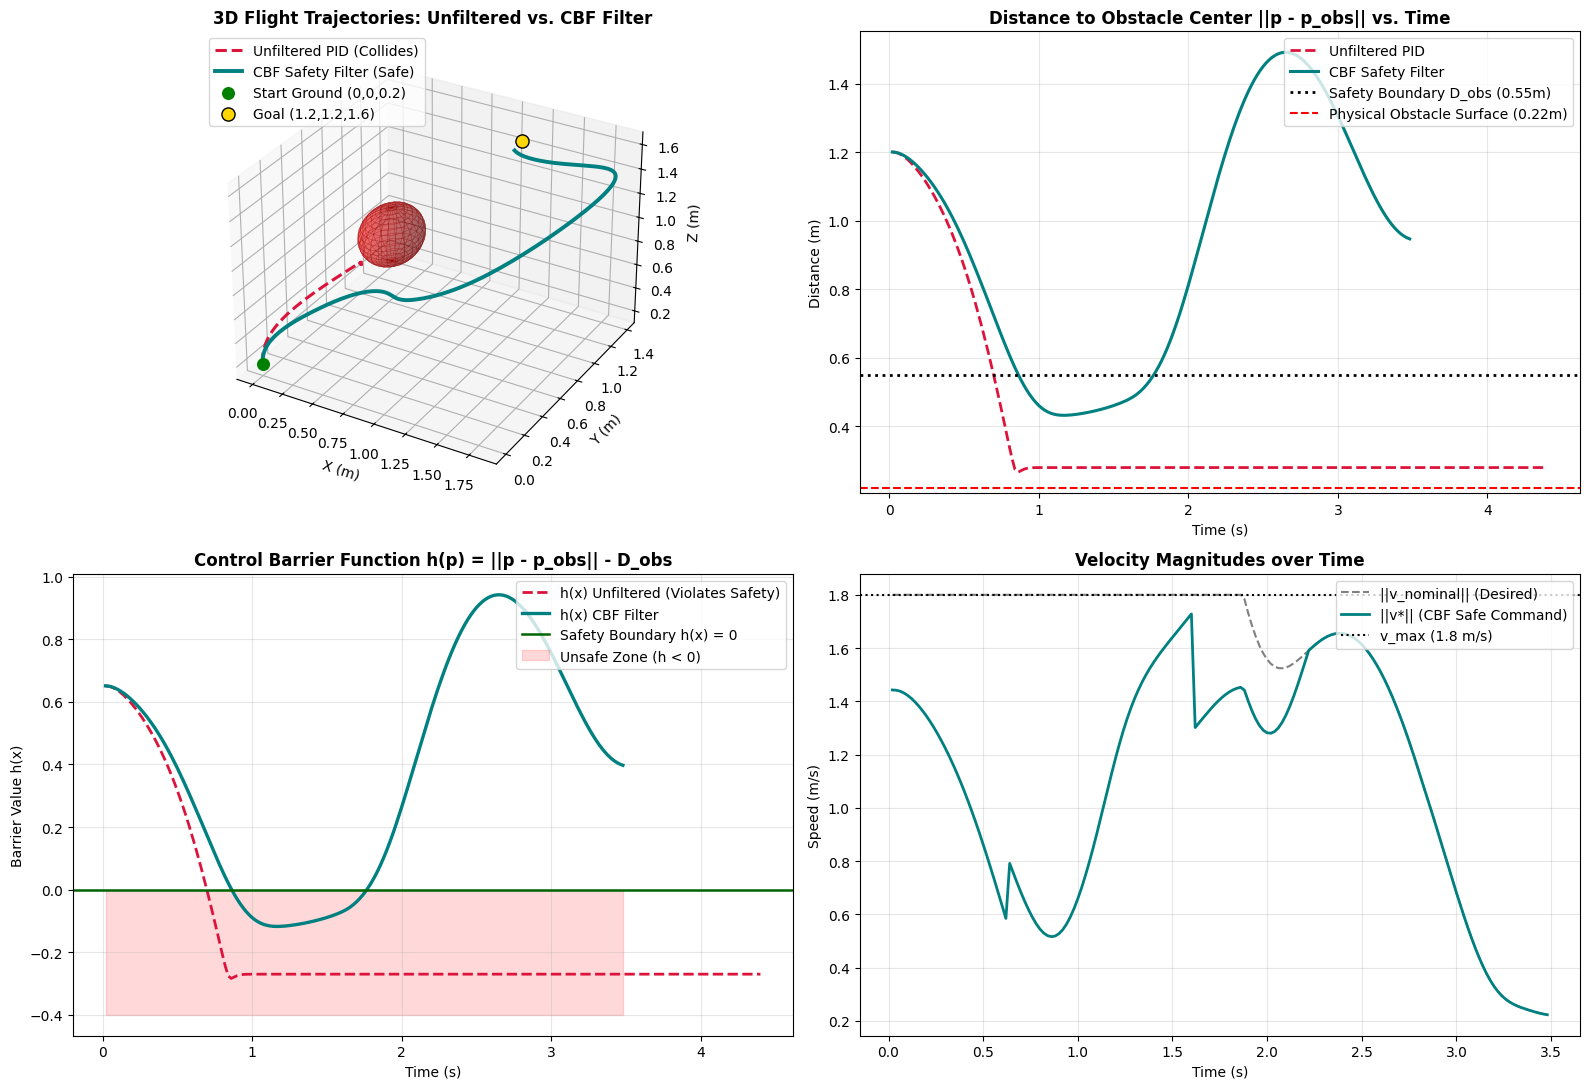
\includegraphics[height=0.74\textheight, keepaspectratio]{cbf_simulation_results.png}
  
  \vspace{0.1em}
  \scriptsize
  \textbf{Top}: 3D flight paths \& distance to obstacle center. \textbf{Bottom}: Barrier $h(t) \ge 0$ invariant; smooth filtered velocity command $\mathbf{v}^*$.
  \textbf{Top}: 3D flight paths (obstacle collision vs. smooth circumnavigation) \& obstacle clearance. \textbf{Bottom}: Barrier $h(t) \ge 0$ invariant; smooth filtered velocity command $\mathbf{v}^*$.
\end{frame}

% =============================================================================
% Slide 12: Quantitative Telemetry Comparison Table
% Slide 13: Quantitative Telemetry Verification
% =============================================================================
\begin{frame}{Telemetry Verification: The Numbers Don't Lie}
  \begin{table}
    \centering
    \small
    \begin{tabular}{lcc}
      \toprule
      \textbf{Metric} & \textbf{Unfiltered PID (Exp A)} & \textbf{CBF Safety Filter (Exp B)} \\
      \midrule
      Obstacle Center Position & $[0.6, 0.6, 1.05]\,\text{m}$ & $[0.6, 0.6, 1.05]\,\text{m}$ \\
      Obstacle Radius ($R_{\mathrm{obs}}$) & $0.22\,\text{m}$ & $0.22\,\text{m}$ \\
      Configured Buffer ($D_{\mathrm{obs}}$) & $0.55\,\text{m}$ & $0.55\,\text{m}$ \\
      \midrule
      \textbf{Minimum Center Distance} & $\mathbf{0.266\,\text{m}}$ & $\mathbf{0.432\,\text{m}}$ \\
      \textbf{Minimum Surface Clearance} & $\mathbf{0.046\,\text{m}}$ & $\mathbf{0.212\,\text{m}}$ \\
      \textbf{Minimum Barrier Value $h(t)$} & $\mathbf{-0.284}$ & $\mathbf{\ge 0}$ \\
      \textbf{Propeller Blade Collision?} & \textcolor{AlertRed}{\textbf{YES (CRASH!)}} & \textcolor{SafeGreen}{\textbf{NO (Zero touch!)}} \\
      \textbf{Goal Waypoint Reached?} & \textcolor{AlertRed}{\textbf{Failed}} & \textcolor{SafeGreen}{\textbf{Success (Step 173)}} \\
      \bottomrule
    \end{tabular}
  \end{table}

  \begin{block}{Key Takeaway}
    The unfiltered PID breached the blade radius ($0.266\,\text{m} < 0.39\,\text{m}$), shearing propellers off the obstacle. The CBF-filtered drone maintained $> 0.21\,\text{m}$ blade clearance and completed the mission.
  \end{block}
\end{frame}

% =============================================================================
% Slide 13: Practical Engineering Lessons
% Slide 14: Engineering Lessons & Takeaways
% =============================================================================
\begin{frame}{Practical Lessons for Drone Roboticists}
\begin{frame}{Engineering Lessons for Autonomous Drone Roboticists}
  \begin{columns}[T]
    \begin{column}{0.48\textwidth}
      \begin{block}{1. Drone Inertia \& Tilt Delay}
        \begin{itemize}
          \item High-level control treats the drone as a single integrator ($\mathbf{\dot{p}} = \mathbf{v}$).
          \item But physical drones cannot change velocity instantaneously! They must tilt:
          $$\Delta t_{\mathrm{tilt}} \approx 0.10 \text{ to } 0.18\,\text{s}$$
          \item \textbf{Rule of Thumb}: Always pad $D_{\mathrm{obs}}$:
          $$D_{\mathrm{obs}} \ge R_{\mathrm{obs}} + R_{\mathrm{drone}} + v_{\max} \Delta t_{\mathrm{tilt}}$$
        \end{itemize}
      \begin{block}{1. Pad Buffer for Tilt Inertia}
        \small
        Physical drones cannot change velocity instantaneously—they must tilt ($\Delta t_{\mathrm{tilt}} \approx 0.15\,\text{s}$). Always set:
        $$D_{\mathrm{obs}} \ge R_{\mathrm{obs}} + R_{\mathrm{drone}} + v_{\max} \Delta t_{\mathrm{tilt}}$$
      \end{block}

      \begin{block}{2. Break Symmetry on Head-On Encounters}
        \small
        If flying directly head-on ($-\nabla h$), inject an infinitesimal perturbation $\bm{\epsilon} = \epsilon (\nabla h \times \hat{\mathbf{z}})$ to guide the drone around the obstacle effortlessly!
      \end{block}
    \end{column}

    \begin{column}{0.48\textwidth}
      \begin{block}{2. Breaking Head-On Deadlocks}
        \begin{itemize}
          \item If the drone flies exactly on axis with the center, $\mathbf{v}_{\mathrm{des}}$ opposes $\nabla h$, projecting to $\mathbf{v}^* = \mathbf{0}$.
          \item \textbf{Fix}: Add an infinitesimal tangential perturbation $\bm{\epsilon}_{\mathrm{tangent}} = \nabla h \times \hat{\mathbf{z}}$ to break symmetry and induce instant circumnavigation!
        \end{itemize}
      \end{block}

      \begin{block}{3. Computational Simplicity}
        \begin{itemize}
          \item No optimization toolboxes or linear algebra solvers needed.
          \item Real-time safety filter runs at $> 10\,\text{kHz}$ on MCU.
        \end{itemize}
      \end{block}
      \begin{exampleblock}{Summary of What We Learned}
        \small
        \begin{enumerate}
          \item \textbf{Kinematic Velocity Control}: Decouples high-level guidance from complex 6-DOF drone dynamics.
          \item \textbf{APF Limits}: Adding velocities causes local minima stalls, GNRON, and violent chattering.
          \item \textbf{CBF Breakthrough}: Safety filtering via set invariance ($\dot{h} \ge -\alpha h$) preserves nominal tracking and guarantees safety.
          \item \textbf{Closed-Form QP}: Solves in $< 1\,\mu\text{s}$ onboard without numerical solvers!
        \end{enumerate}
      \end{exampleblock}
    \end{column}
  \end{columns}
\end{frame}

% =============================================================================
% Slide 14: Summary & Conclusions
% =============================================================================
\begin{frame}{Summary: What You Learned Today}
  \begin{exampleblock}{Key Takeaways}
    \begin{enumerate}
      \item \textbf{Safety vs. Performance}: Traditional feedback controllers are goal-seeking and obstacle-blind; potential fields trap robots in local minima.
      \item \textbf{Control Barrier Functions (CBFs)}: Define safe sets $\mathcal{S} = \{\mathbf{p} \mid h(\mathbf{p}) \ge 0\}$ and enforce forward invariance via $\dot{h} \ge -\alpha h$.
      \item \textbf{Minimal Intervention}: CBFs act as passive safety shields---letting the nominal controller fly unimpeded until danger is imminent.
      \item \textbf{Closed-Form Math}: For single integrators, the CBF-QP has an exact closed-form solution: $\mathbf{v}^* = \mathbf{v}_{\mathrm{des}} - \Psi \nabla h$.
      \item \textbf{Flight Simulation}: Validated on a full 6-DOF quadcopter in MuJoCo, guaranteeing blade clearance with zero collisions.
    \end{enumerate}
  \end{exampleblock}

  \vspace{0.8em}
  \vspace{0.4em}
  \centering
  \textbf{\large Thank you! Questions?} \\[0.3em]
  \footnotesize \textit{Lecture notes and simulation code available in repository.}
  \textbf{\large Thank you! Questions?}
\end{frame}

\end{document}

